%   % !TEX root = ../../VIII,3_Rahmen-TeX_8-1.tex
%
%   Band VIII, 3 N.~??A21.1/Y.2
%   Signatur/Tex-Datei: LH_37_03_069-070,LH_35_09_16_001
%   RK-Nr. 60201
%   Überschrift: De firmitate corporum
%   Datierung: [Ende Januar bis März/April 1683]
%   WZ: RK-WZ 134 = Krone auf eingekreistem Ross mit Gegenmarke AB (zweimal)
%.  SZ: (keins)
%.  Bilddateien (PDF): LH_37_03_069-070_d01; LH_37_03_069-070_d02; LH_37_03_069-070_d03; LH_37_03_069-070_d04; LH_37_03_069-070_d05; LH_37_03_069-070_d06; LH_37_03_069-070_d07; LH_37_03_069-070_d08; LH_37_03_069-070_d09; LH_37_03_069-070_d10; LH_37_03_069-070_d11; LH_37_03_069-070_d12a; LH_37_03_069-070_d12b; LH_37_03_069-070_d12c; LH_35_09_16_001_d13 (insgesamt: fünfzehn)
%
%
\selectlanguage{ngerman}%
\frenchspacing%
%
\begin{ledgroupsized}[r]{120mm}
\footnotesize
\pstart
\noindent\textbf{Überlieferung:}
\pend
\end{ledgroupsized}
\begin{ledgroupsized}[r]{114mm}
\footnotesize
\pstart \parindent -6mm
\makebox[6mm][l]{\textit{L}}%
Konzept: LH~XXXV~9,~16 Bl.~1,~20 und LH~XXXVII~3 Bl.~69\textendash70.
Zwei Bogen 2\textsuperscript{o};
% gleiche Wasserzeichen und Gegenmarken auf beiden Bogen.
gleiches Wasserzeichen auf Bl.~1 und 70 mit Gegenmarke auf Bl.~20 und 69:
Papier aus dem Harz;
Textverlust am unteren Rand von Bl.~70~v\textsuperscript{o}.
Fünf Seiten und vier Zeilen;
Textfolge (nicht von Leibniz festgelegt):
% Bl.~69, 70 und 1;
Bl.~69~r\textsuperscript{o}, 69~v\textsuperscript{o}, 70~r\textsuperscript{o}, 70~v\textsuperscript{o}, 1~r\textsuperscript{o} und 1~v\textsuperscript{o};
Text von Bl.~70~v\textsuperscript{o} (mittig) an gestrichen; % durchgängig 
% LH~XXXV~9,~16 
auf Bl.~1~v\textsuperscript{o} bis Bl.~20~v\textsuperscript{o} ist N.~14\textsubscript{3} überliefert.
Der Abschnitt \textit{Experientia notum} \lbrack...\rbrack\ \textit{aere libero} (S.~\refpassage{LH_37_03_069r_duaetabulae-1}{LH_37_03_069r_duaetabulae-2}) ist in N.~14\textsubscript{5} %, S.~\refpassage{LH037_03_118r_wiedergabe-1}{LH037_03_118r_wiedergabe-2} 
wiedergegeben.
\pend
\end{ledgroupsized}
%
%
\selectlanguage{latin}%
\frenchspacing%
%
%
\vspace{8mm}
%
%
\count\Bfootins=1000
\count\Afootins=1100
\count\Cfootins=1100
%
% 
\pstart%
\normalsize%
\noindent%
%
\lbrack69~r\textsuperscript{o}\rbrack\ % Bl. 69r
%
\pend%
%\vspace{-0.5em}%
%
% Überschrift
\pstart%
\centering%
\edtext{De firmitate corporum\protect\index{Sachverzeichnis}{firmitas corporis}}{%
\lemma{De}\Bfootnote{%
\textit{(1)}~resistentia\protect\index{Sachverzeichnis}{resistentia solidi}
\textit{(a)}~solidorum
\textit{(b)}~corporum\protect\index{Sachverzeichnis}{resistentia corporis}
\textit{(2)}~corporum fir
\textit{(3)}~firmitate corporum%
~\textit{L}}}
\pend%
\vspace{0.5em}%
%
\pstart%
\noindent%
Partes solidorum\protect\index{Sachverzeichnis}{partes solidorum} duobus
\edtext{modis\protect\index{Sachverzeichnis}{modus connexionis}
connexae\protect\index{Sachverzeichnis}{partes connexae}
inter se intelliguntur.
Vi enim adhibita\protect\index{Sachverzeichnis}{vis adhibita}}{%
\lemma{modis}\Bfootnote{%
\textit{(1)}~connceti inter se intelligi possunt.
\textit{(2)}~connexae inter se intelliguntur.
\textit{(a)}~Vis enim connectens\protect\index{Sachverzeichnis}{vis connectens}
\textit{(b)}~Vi enim adhibita%
~\textit{L}}}
%
vel a se
\edtext{invicem}{%
\lemma{invicem}\Bfootnote{%
\textit{erg.~L}}}
%
possunt nonnihil recedere,
salva earum
\edtext{cohaesione,\protect\index{Sachverzeichnis}{cohaesio partium}
ut cum filum\protect\index{Sachverzeichnis}{filum tensum} tendimus aut}{%
\lemma{cohaesione,}\Bfootnote{%
\textit{(1)}~vel ut
\textit{(2)}~ut cum filum tendimus aut%
~\textit{L}}}
%
cum baculum flectimus;\protect\index{Sachverzeichnis}{baculus flexus}
\edtext{vel non possunt a se invicem tantillum recedere, quin statim abrumpantur,
ut fit cum duae tabulae politae\protect\index{Sachverzeichnis}{tabula polita}
sibi applicatae divelluntur\lbrack,\rbrack\
si fingamus aerem subintrare\protect\index{Sachverzeichnis}{aer subintrans} ubi tantillum a se recesserint.}{%
\lemma{vel}\Bfootnote{%
\textit{(1)}~si quam minimum a se invicem recedant
\textit{(2)}~non
\textit{(a)}~sunt
\textit{(b)}~possunt a se
\textit{(aa)}~vel
\textit{(bb)}~invicem tantillum recedere, quin statim
\textit{(aaa)}~frangantur,
\textit{(aaaa)}~ut glacies et vitrum,\protect\index{Sachverzeichnis}{glacies}\protect\index{Sachverzeichnis}{vitrum}
\textit{(aaaaa)}~saltem ad sensu\lbrack\textit{!}\rbrack\
\textit{(bbbbb)}~quae saltem
\textit{(ccccc)}~quae tamen et ipsa aliquid f
\textit{(bbbb)}~quod sensus de glacie aut vitro crassiusculis testari videtur, licet
\textit{(bbb)}~abrumpantur, ut fit
\textit{(aaaa)}~si
\textit{(bbbb)}~cum duae \lbrack...\rbrack\ sibi applicatae % tabulae politae
\textit{(aaaaa)}~divellantur
\textit{(bbbbb)}~divelluntur
\textit{(aaaaa-a)}~.
\textit{(bbbbb-b)}~si
\textit{(aaaaa-aa)}~ponamus
\textit{(bbbbb-bb)}~fingamus aerem \lbrack...\rbrack\ se recesserint.% subintrare ubi tantillum a
~\textit{L}}}
%
De posteriori autem connexionis modo,\protect\index{Sachverzeichnis}{modus connexionis}
cum sit simplicior, prius dicemus.
\edtext{}{{\xxref{LH_37_03_069r_duaetabulae-1}{LH_37_03_069r_duaetabulae-2}}%
{\lemma{Experientia \lbrack...\rbrack\ libero}\Cfootnote{%
In N.~14\textsubscript{5}, S.~\refpassage{LH037_03_118r_wiedergabe-1}{LH037_03_118r_wiedergabe-2} wiedergegeben.}}}%
%
\edtext{Experientia\edlabel{LH_37_03_069r_duaetabulae-1}%
\protect\index{Sachverzeichnis}{experientia}
notum}{%
\lemma{Experientia notum}\Cfootnote{% 
Siehe etwa G.~\textsc{Galilei}, \textit{Discorsi}, Leiden 1638, S.~12\cite{00050} (\textit{GO} VIII, S.~59.13\textendash23);\cite{00048}
P.~\textsc{Gassendi}, \textit{Physica}, sectio~I, lib.~II, cap.~IV\cite{01073} (\textit{GOO} I, S.~202a).\cite{01029}}}
%
est duas
\edtext{Tabulas planas\protect\index{Sachverzeichnis}{tabula plana}}{%
\lemma{Tabulas planas}\Cfootnote{%
Siehe \lbrack\textit{Fig.~1}\rbrack\ auf S.~\pageref{LH_37_03_069r_Fig.1}.}}
%
\textit{AB} et \textit{CD}
firmas,\protect\index{Sachverzeichnis}{tabula firma} ac bene
\edtext{politas,\protect\index{Sachverzeichnis}{tabula polita}
politisque superficiebus\protect\index{Sachverzeichnis}{superficies tabulae}
sibi applicatas\protect\index{Sachverzeichnis}{tabulae sibi applicatae}}{%
\lemma{politas,}\Bfootnote{%
\textit{(1)}~ita sibi a
\textit{(2)}~ac politis
\textit{(3)}~politisque superficiebus sibi applicatas%
~\textit{L}}}
%
difficulter a se invicem avelli,
quanquam manente earum applicatione facile una super alia incedere possit.
Cau- \makebox[1.0\textwidth][s]{sa\protect\index{Sachverzeichnis}{causa adhaesionis} esse potest vel a
\edtext{pondere\protect\index{Sachverzeichnis}{pondus tabulae} aut}{%
\lemma{pondere}\Bfootnote{%
\textit{(1)}~et
\textit{(2)}~aut%
~\textit{L}}}
%
elastro aeris\protect\index{Sachverzeichnis}{elastrum aeris}
alteriusve corporis liquidi aut solidi in eas}
\pend
\newpage
\pstart
\noindent tabulas nitentis;
vel etiam aliquando a sola
\edtext{plenitudine loci\protect\index{Sachverzeichnis}{plenitudo loci}
ambientis\protect\index{Sachverzeichnis}{locus ambiens}}{%
\lemma{plenitudine}\Bfootnote{%
\textit{(1)}~rerum li
\textit{(2)}~loci ambientis%
~\textit{L}}}
%
probe clausi.\protect\index{Sachverzeichnis}{locus clausus}
% \edtext{}{%
% {\xxref{LH_37_03_069r_invase-1}{LH_37_03_069r_invase-2}}%
% {\lemma{%
% Ut si \lbrack...\rbrack\ obturato}\Cfootnote{%
% Siehe \lbrack\textit{Fig.~1}\rbrack\ auf S.~\pageref{LH_37_03_069r_Fig.1}.}}}%
%
\edlabel{LH_37_03_069r_invase-1}Ut
\edtext{si in vase\protect\index{Sachverzeichnis}{vas obturatum} firmissimo perfecte obturato,\edlabel{LH_37_03_069r_invase-2}
et aqua ita pleno,\protect\index{Sachverzeichnis}{vas aqua plenum}}{%
\lemma{si}\Bfootnote{%
\textit{(1)}~in vase aqua pleno perfectissime clauso, vi 
\textit{(2)}~in vase firmissimo perfecte
\textit{(a)}~clauso, et
\textit{(b)}~obturato, et aqua ita pleno,%
~\textit{L}}}
%
ut nec unica eius gutta\protect\index{Sachverzeichnis}{gutta}
\edtext{amplius immitti}{%
\lemma{amplius}\Bfootnote{%
\hspace{-0,5mm}\textbar~ulla \textit{gestr.}~%
\textbar\ immitti%
~\textit{L}}}
%
possit,
hae duae
\edtext{Tabulae}{%
\lemma{Tabulae}\Bfootnote{%
\textit{erg.~L}}}
%
sibi applicatae\protect\index{Sachverzeichnis}{tabulae sibi applicatae} sint,
tunc posito nihil nisi aquam intus esse,
et aquam esse compressionis\protect\index{Sachverzeichnis}{compressio aquae} incapacem,
et
\edtext{tabularum planitiem\protect\index{Sachverzeichnis}{planities tabulae} esse exactam,
firmitatemque tabularum\protect\index{Sachverzeichnis}{firmitas tabulae}
pariter et vasis\protect\index{Sachverzeichnis}{firmitas vasis}}{%
\lemma{tabularum}\Bfootnote{%
\textit{(1)}~vasisque
\textit{(2)}~planitiem esse \lbrack...\rbrack\ et vasis% % exactam, firmitatemque tabularum pariter
~\textit{L}}}
%
\edtext{insuperabilem; nulla}{%
\lemma{insuperabilem;}\Bfootnote{% 
\hspace{-0,5mm}\textbar~tunc \textit{erg. u. gestr.}~%
\textbar\ nulla%
~\textit{L}}}
%
vi tabulae poterunt
\edtext{divelli:\protect\index{Sachverzeichnis}{vis divellendi}
interstitium\protect\index{Sachverzeichnis}{interstitium} enim quantulumcunque
uno momento\protect\index{Sachverzeichnis}{momentum temporis}
a fluido irruente\protect\index{Sachverzeichnis}{fluidum irruens} impleri impossibile est.}{%
\lemma{divelli}\Bfootnote{%
\textit{(1)}~.
\textit{(2)}~: interstitium enim \lbrack...\rbrack\ uno momento % quantulumcunque
\textit{(a)}~ab aqua
\textit{(b)}~a fluido \lbrack...\rbrack\ impossibile est.% % irruente impleri
~\textit{L}}}
%
Nunc autem cum omnia nonnihil cedant,
poterunt divelli aliqua sane vi,\protect\index{Sachverzeichnis}{vis divellendi}
\edtext{sed necessario longe majore,}{%
\lemma{sed}\Bfootnote{%
\textit{(1)}~longe majore,
\textit{(2)}~necessario longe majore,%
~\textit{L}}}
%
quam in aere\protect\index{Sachverzeichnis}{aer liber}
\edtext{libero.%
\edlabel{LH_37_03_069r_duaetabulae-2}
Nos autem}{%
\lemma{libero.}\Bfootnote{%
\textit{(1)}~Sed nos
\textit{(2)}~Nos autem%
~\textit{L}}}
%
hoc loco de causa\protect\index{Sachverzeichnis}{causa adhaesionis}
\edtext{non}{%
\lemma{non}\Bfootnote{%
\textit{erg.~L}}}
%
solliciti,
effectus\protect\index{Sachverzeichnis}{effectus} tantum considerabimus,
et consequentias,\protect\index{Sachverzeichnis}{consequentia}
\edtext{si solidorum Corporum\protect\index{Sachverzeichnis}{corpus solidum}
partes\protect\index{Sachverzeichnis}{partes solidorum} hoc modo}{%
\lemma{si}\Bfootnote{%
\textit{(1)}~solida hoc m
\textit{(2)}~solidorum Corporum partes hoc modo%
~\textit{L}}}
%
compactae\protect\index{Sachverzeichnis}{modus connexionis} intelligantur.%
%%    %%    %%    %%        A C H T U N G   G E T R I X T       !!    !!    !!    !!
\edtext{}{\lemma{\hspace*{1,6mm}\lbrack\textit{Fig.~1}\rbrack}\killnumber\Cfootnote{%
Das Diagramm ist in \textit{L} von einem gestrichenen, hier nicht wiedergegebenen Entwurf begleitet.}}
%
\pend%
%
%
%
%
 \pstart%
Ponamus\edlabel{LH_37_03_069r_rupturadirecta-1} autem
\edtext{vim}{%
\lemma{vim}\Bfootnote{%
\textit{erg.~L}}}
%
divellentem\protect\index{Sachverzeichnis}{vis divellens}
\edtext{niti in recta perpendiculari\protect\index{Sachverzeichnis}{nisus perpendicularis}}{%
\lemma{niti}\Bfootnote{%
\textit{(1)}~perpendiculariter
\textit{(2)}~in \textbar~linea \textit{gestr.}~\textbar\ recta perpendiculari%
~\textit{L}}}
%
\edtext{ad superficies}{%
\lemma{ad}\Bfootnote{%
\textit{(1)}~superficiem
\textit{(2)}~superficies%
~\textit{L}}}
%
divellendas,\protect\index{Sachverzeichnis}{superficies divellenda}
\edtext{ut in rectis
\edtext{\textit{eg} vel \textit{fh},}{%
\lemma{\textit{eg}}\Bfootnote{%
\textit{(1)}~\textit{fh},
\textit{(2)}~vel \textit{fh},%
~\textit{L}}}%
}{\lemma{ut \lbrack...\rbrack\ \textit{fh}}\Cfootnote{%
Siehe \lbrack\textit{Fig.~2}\rbrack\ auf S.~\pageref{LH_37_03_069r_Fig.2}.}}
%
et vim divellendi\protect\index{Sachverzeichnis}{vis divellendi}
applicatam esse ad puncta \textit{e} vel \textit{f},\hspace{0.3mm}
centra\protect\index{Sachverzeichnis}{centrum gravitatis tabulae}
\edtext{\hspace{0.3mm}gravitatis\hspace{0.3mm} superficiei\hspace{0.3mm}}{%
\lemma{gravitatis}\Bfootnote{%
\textit{(1)}~superficierum
\textit{(2)}~superficiei%
~\textit{L}}}
%
communis\hspace{0.3mm} tabularum\hspace{0.3mm} divellendarum,\protect\index{Sachverzeichnis}{tabula divellenda}
\edtext{\hspace{0.3mm}tunc}{%
\lemma{tunc}\Bfootnote{%
\textit{erg.~L}}}
%
manifestum\hspace{0.3mm} est\lbrack:\rbrack\ 
\edtext{\hspace{0.3mm}si\hspace{0.3mm} tabulae\hspace{0.3mm} sint\hspace{0.3mm} rigidae\hspace{0.3mm}\protect\index{Sachverzeichnis}{tabula rigida}}{% \lbrack,\rbrack
\lemma{si}\Bfootnote{%
\hspace{-0,5mm}tabulae sint rigidae
\textit{erg.~L}}}
%
nullum\hspace{0.3mm} locum\hspace{0.3mm} prae\hspace{0.2mm} alio\hspace{0.2mm} laborare,\hspace{0.2mm} sed\hspace{0.2mm} divulsionem\protect\index{Sachverzeichnis}{divulsio tabulae}\hspace{0.2mm} in\hspace{0.2mm} omnibus\hspace{0.2mm} aeque
\pend
%%%%%%%%%%%%%%%%%%%%%%%Abbildung 1%%%%%%%%%%%%%%%%%%%%%%%%%%%%%%%%%%%%%%%%%%%%%%%
 \vspace{1.2em}%
  \centerline{\includegraphics[width=0.33\textwidth]{gesamttex/edit_VIII,3/images/LH_37_03_069-070_d01.pdf}}% 
  \vspace{0.5em}
  \centerline{\lbrack\textit{Fig.~1}\rbrack}\label{LH_37_03_069r_Fig.1}%
\newpage
%%%%%%%%%%%%%%%%%%%%%%%%Abbildung 2 und 3 %%%%%%%%%%%%%%%%%%%%%%%%%%%%%%%%%%%%%%%%%%%%%%%
\pstart
\hspace{5mm}\begin{minipage}[t]{0.5\textwidth}
\includegraphics[width=0.57\textwidth]{gesamttex/edit_VIII,3/images/LH_37_03_069-070_d02.pdf}
\end{minipage}
\hspace{0mm}
\begin{minipage}[t]{0.5\textwidth}
\includegraphics[width=0.55\textwidth]{gesamttex/edit_VIII,3/images/LH_37_03_069-070_d03.pdf}
\end{minipage}
\\
\\
%\vspace*{1em}
\hspace*{24  mm} [\textit{Fig.~2}] \label{LH_37_03_069r_Fig.2}\hspace{57mm} [\textit{Fig.~3}] \label{LH_37_03_069r_Fig.3}
\pend
\vspace{1.5em}
\pstart
\noindent inchoari;\setline{1} manifestum
\edtext{est quoque vim\protect\index{Sachverzeichnis}{vis avulsura}
quae avulsura sit}{%
\lemma{est}\Bfootnote{%
\hspace{-0,5mm}\textbar~quoque \textit{erg.}~\textbar\
\textit{(1)}~vires
\textit{(2)}~vim
\textit{(a)}~quae divulsura sit
\textit{(b)}~quae avulsura sit%
~\textit{L}}}
%
tabulam \textit{f} a tabula \textit{CD},
fore ad vim quae avulsura sit \textit{e} ab
\edtext{eadem \textit{CD},}{%
\lemma{eadem}\Bfootnote{%
\textit{(1)}~\textit{ED},
\textit{(2)}~\textit{CD},%
~\textit{L}}}
%
ut
\edtext{tabulae \textit{f} superficies communis\protect\index{Sachverzeichnis}{superficies communis}}{%
\lemma{tabulae \textit{f}}\Bfootnote{%
\textit{(1)}~superficiem communem
\textit{(2)}~superficies communis%
~\textit{L}}}\protect\index{Sachverzeichnis}{superficies divellenda}
%
cum tabula \textit{CD},
\edtext{est}{%
\lemma{est}\Bfootnote{%
\textit{erg.~L}}}
%
ad superficiem communem\protect\index{Sachverzeichnis}{superficies communis}
tabulae \textit{e} cum\protect\index{Sachverzeichnis}{superficies tabulae}
\edtext{eadem \textit{CD}, seu}{%
\lemma{eadem}\Bfootnote{%
\hspace{-0,5mm}\textbar~\textit{CD}, \textit{erg.}~\textbar\ seu%
~\textit{L}}}
%
vires\protect\index{Sachverzeichnis}{vis directe divellens}
\edtext{directe per centrum}{%
\lemma{directe}\Bfootnote{%
\textit{(1)}~ex centro
\textit{(2)}~per centrum%
~\textit{L}}}
%
divellentes esse inter se ut superficies\protect\index{Sachverzeichnis}{superficies divellenda} communes.\edlabel{LH_37_03_069r_rupturadirecta-2}
\pend%
%
%%
%  \vspace*{3.0em}%
%  \centerline{\hspace*{-70mm}\includegraphics[width=0.28\textwidth]{gesamttex/edit_VIII,3/images/LH_37_03_069-070_d02.pdf}}%
%  \vspace*{-1.0em}
%  \centerline{\hspace*{-70mm}\lbrack\textit{Fig.~2}\rbrack}%
%  \label{LH_37_03_069r_Fig.2}%
%%
%%  \newpage
%  \vspace*{-11.0em}%
%  \centerline{\hspace*{65mm}\includegraphics[width=0.29\textwidth]{gesamttex/edit_VIII,3/images/LH_37_03_069-070_d03.pdf}}% 
%  \vspace*{-1.0em}
%  \centerline{\hspace*{75mm}\lbrack\textit{Fig.~3}\rbrack}%
%  \label{LH_37_03_069r_Fig.3}%
%  \vspace*{1.5em}%
%
%
\pstart%
% % % %    ACHTUNG GETRIXT    ! ! ! ! 
% \edtext{}{\lemma{\hspace{1,6mm}\lbrack\textit{Fig.~3}\rbrack}\killnumber\Cfootnote{Das Diagramm ist perspektivisch nicht korrekt.}}
Est vero alius divellendi nisus
quem vocabo circularem,\protect\index{Sachverzeichnis}{nisus divellendi circularis}
\edtext{ut si ponatur Tabula plana \textit{CD}\protect\index{Sachverzeichnis}{tabula plana}}{%
\lemma{ut \lbrack...\rbrack\ \textit{CD}}\Cfootnote{%
Siehe \lbrack\textit{Fig.~3}\rbrack.}}
%
verticaliter erecta,
eique\protect\index{Sachverzeichnis}{tabulae sibi applicatae}
\edtext{applicata sit recta \textit{GHL}}{%
\lemma{applicata}\Bfootnote{%
\textit{(1)}~linea
\textit{(a)}~nem 
\textit{(b)}~\textbar~recta \textit{erg.}~\textbar\ \textit{g}\textlangle\textit{hl}\textrangle\
\textit{(2)}~sit recta \textit{GHL}%
~\textit{L}}}
%
horizonti parallela,
cujus latitudinem hoc loco non considerabimus,
ex cujus medio demittatur perpendicularis
\edtext{\lbrack\textit{HA}\rbrack}{%
\lemma{\textit{hA}}\Bfootnote{%
\textit{L~ändert Hrsg.}}}
%
et ex \textit{A} educatur ad tabulam \textit{CD} normalis \textit{AM},
sitque angulus rectus\protect\index{Sachverzeichnis}{angulus rectus mobilis}
\textit{HAM} mobilis circa centrum \textit{A},
una cum linea \textit{GL}
\edtext{affixa in \textit{H},
a nisu ponderis \textit{N}\protect\index{Sachverzeichnis}{nisus ponderis}
appensi\protect\index{Sachverzeichnis}{pondus appensum} in \textit{M},
tunc\textso{ nisum }%
quo vis\protect\index{Sachverzeichnis}{vis avellendi}}{%
\lemma{affixa}\Bfootnote{% 
\hspace{-0,5mm}\textbar~in \textit{H}, \textit{erg.}~\textbar\
\textit{(1)}~tunc is nisus quo po
\textit{(2)}~a nisu \lbrack...\rbrack\ quo vis%
~\textit{L}}}
%
lineam \textit{GL} a tabula \textit{CD} avellere
\edtext{conatur voco}{%
\lemma{conatur}\Bfootnote{%
\textit{(1)}~vocabo
\textit{(2)}~voco%
~\textit{L}}}%
%
\textso{ circularem,}
\protect\index{Sachverzeichnis}{nisus avellendi circularis}\protect\index{Sachverzeichnis}{vectis}%
vel etiam\textso{ per vectem,}
\edtext{praecedentibus}{%
\lemma{praecedentibus}\Cfootnote{%
Vgl. S.~\refpassage{LH_37_03_069r_rupturadirecta-1}{LH_37_03_069r_rupturadirecta-2}.}}
%
\edtext{vero explicatum}{%
\lemma{vero}\Bfootnote{%
\textit{(1)}~applicatam
\textit{(2)}~explicatum%
~\textit{L}}}
%
voco\textso{ }%
\edtext{}{{\xxref{KZeitz167}{KZeitz168}}%
{%
\lemma{\textso{directum}}\Bfootnote{%
\textit{(1)}~. Quods
\textit{(2)}~. Ubi primum noto: Nisum circularem
\textit{(a)}~pond
\textit{(b)}~si \textit{AM} et \textit{AH} sint aeq
\textit{(3)}~qualem
\textit{(a)}~exercet
\textit{(b)}~exerceret 
\textit{(c)}~pondus \textit{P}
\textit{(aa)}~, ut autem
\textit{(bb)}~exerceret, si vi ejus %
\textbar~linea \textit{erg.}~\textbar\ \textit{GL} avellenda \lbrack...\rbrack\ \textit{AM}, ita
\textit{(aaa)}~vim resisten
\textit{(bbb)}~vinculum quod
\textit{(aaaa)}~\textit{GL}
\textit{(bbbb)}~lineam \textit{GL}
\textit{(aaaaa)}~annectit
\textit{(bbbbb)}~Tabulae annectit, \lbrack...\rbrack\ nisum circularem%
~\textit{L}}}}%
\edlabel{KZeitz167}\textso{directum}\textso{ }%
\protect\index{Sachverzeichnis}{nisus divellendi directus}qualem pondus \textit{P} exerceret,\protect\index{Sachverzeichnis}{pondus appensum}
si vi ejus linea \textit{GL} avellenda esset.\protect\index{Sachverzeichnis}{vis avellendi}
Ubi primum noto\lbrack:\rbrack\
ut pondus \textit{N}\protect\index{Sachverzeichnis}{pondus appensum}
nititur agere per vectem \textit{AM},\protect\index{Sachverzeichnis}{vectis}
\makebox[1.0\textwidth][s]{ita vinculum\protect\index{Sachverzeichnis}{vinculum}
quod lineam \textit{GL} Tabulae\protect\index{Sachverzeichnis}{tabula rigida} annectit,
vicissim resistere per vectem contrarium}
\pend
\newpage
\pstart
\noindent \textit{AH}.\protect\index{Sachverzeichnis}{vectis contrarius}
Et proinde si vectis\protect\index{Sachverzeichnis}{vectis}
et vectis contrarius\protect\index{Sachverzeichnis}{vectis contrarius} sint aequales\lbrack,\rbrack\
nisum circularem\protect\index{Sachverzeichnis}{nisus divellendi circularis}\edlabel{KZeitz168}
%
aequipollere directo,\protect\index{Sachverzeichnis}{nisus divellendi directus}
\edtext{sive pondera\protect\index{Sachverzeichnis}{pondus appensum}}{%
\lemma{sive}\Bfootnote{%
\textit{(1)}~pond
\textit{(2)}~posito
\textit{(3)}~pondus
\textit{(4)}~pondera%
~\textit{L}}}
%
\textit{P} et \textit{N} aequalia idem omnino esse effectura.
Atque
\edtext{hinc habita comparatione\protect\index{Sachverzeichnis}{comparatio nisuum} unius nisus circularis cum directo,%
\protect\index{Sachverzeichnis}{nisus divellendi directus}\protect\index{Sachverzeichnis}{nisus divellendi circularis}
habetur}{%
\lemma{hinc}\Bfootnote{%
\textit{(1)}~facile
\textit{(2)}~habetur
\textit{(3)}~comparatio nisus circul
\textit{(4)}~habita comparatione \lbrack...\rbrack\ directo, habetur% % unius nisus circularis cum
~\textit{L}}}
omnium;
\edtext{nam omnes}{%
\lemma{nam}\Bfootnote{%
\textit{(1)}~caeteri
\textit{(2)}~omnes%
~\textit{L}}}
%
nisus circulares\protect\index{Sachverzeichnis}{nisus divellendi circularis} comparari possunt inter se.
Sunt enim vires\protect\index{Sachverzeichnis}{pondus nitens circulariter}
\edtext{ponderum circulariter nitentium idemque efficientium in reciproca}{%
\lemma{ponderum}\Bfootnote{%
\textit{(1)}~in recipro
\textit{(2)}~circulariter nitentium \lbrack...\rbrack\ in reciproca% % idemque efficientium
~\textit{L}}}
%
vectium\protect\index{Sachverzeichnis}{ratio vectium} ratione,
ut si pondus \textit{R} aeque avellere possit\protect\index{Sachverzeichnis}{pondus avellens}
ac pondus \textit{N},
erit ad ipsum ut \textit{AM} ad \textit{AQ}.
Et proinde erit pondus \textit{R} ad pondus \textit{P}\protect\index{Sachverzeichnis}{pondus avellens}
(\protect\vphantom)%
id est \textit{N}%
\protect\vphantom()
ut \textit{AH}
(\protect\vphantom)%
id est \textit{AM}%
\protect\vphantom()
ad \textit{AQ},
seu pondus circulariter nitens\protect\index{Sachverzeichnis}{pondus nitens circulariter}
est ad
\edtext{\lbrack directe\rbrack}{%
\lemma{directum}\Bfootnote{%
\textit{L~ändert Hrsg.}}}
%
aequipollens,\protect\index{Sachverzeichnis}{pondus nitens directe}
ut
\edtext{vectis resistentiae ad vectem nis\textlangle us.\textrangle}{%
\lemma{vectis}\Bfootnote{%
\textit{(1)}~nisus
\textit{(2)}~resistentiae ad vectem nis\textlangle us.\textrangle%
~\textit{L}}}
%
%
\lbrack69~v\textsuperscript{o}\rbrack\ % Blatt 69v
%
%
\pend%
%
%
\pstart%
Hactenus omnia puncta evellenda aequaliter laboravere % \lbrack,\rbrack\
quoniam
\edtext{vim avellentem\protect\index{Sachverzeichnis}{vis avellens}}{%
\lemma{vim}\Bfootnote{%
\textit{(1)}~appellentem
\textit{(2)}~avellentem%
~\textit{L}}}
%
centro gravitatis omnium applicuimus aequabili erga omnia ratione.
Nunc conjungamus plura puncta inaequaliter resistentia,\protect\index{Sachverzeichnis}{punctum inaequaliter resistens}
non quidem per se,\protect\index{Sachverzeichnis}{per se} sed per accidens\protect\index{Sachverzeichnis}{per accidens}\lbrack,\rbrack\
quia vectis resistentiae\protect\index{Sachverzeichnis}{resistentia vectis} est inaequalis.
Sit ergo \edtext{linea \textit{AE} verticalis}{%
\lemma{linea \textit{AE} verticalis}\Cfootnote{%
Siehe \lbrack\textit{Fig.~4}\rbrack\ auf S.~\pageref{LH_37_03_069v_Fig.4}.}}
%
quae a tabula\protect\index{Sachverzeichnis}{tabula verticalis} \textit{KL}
(\protect\vphantom)%
etiam verticali%
\protect\vphantom()
circulari
% \edtext{}{%
% \lemma{\textit{KL}}\Bfootnote{%
% \textit{(1)}~circula
% \textit{(2)}~(\protect\vphantom)etiam verticali\protect\vphantom()
% circulari%
% ~\textit{L}}}
%
\edtext{nisu\protect\index{Sachverzeichnis}{nisus divellendi circularis} sit avellenda,
pondere aliquo appenso ad vectem \textit{AI};\protect\index{Sachverzeichnis}{pondus vecti appensum}
quod angulum rectum \textit{EAI} moveat\protect\index{Sachverzeichnis}{angulus rectus mobilis}
circa centrum \textit{A}.\protect\index{Sachverzeichnis}{centrum gravitatis tabulae}}{%
\lemma{nisu}\Bfootnote{%
\textit{(1)}~circa centrum scilicet \textit{A},
\textit{(2)}~sit avellenda, pondere \textbar~aliquo \textit{erg.}~\textbar\ appenso ad vectem \textit{AI}
\textit{(a)}~agenteque
\textit{(b)}~\textbar~et \textit{erg.}~\textbar\ circa centrum \textit{A} \textbar~movente \textit{erg.}~\textbar\
\textit{(c)}~; quod angulum \lbrack...\rbrack\ centrum \textit{A}.% % rectum \textit{EAI} moveat circa
~\textit{L}}}
%
Ponamus pondus \textit{M}
\edtext{ope chordae\protect\index{Sachverzeichnis}{chorda} \textit{CQM}}{%
\lemma{ope}\Bfootnote{%
\hspace{-0,5mm}chordae \textit{CQM}
\textit{erg.~L}}}
%
posse lineam \textit{AE} directo nisu
\edtext{a tabula\protect\index{Sachverzeichnis}{tabula verticalis}}{%
\lemma{a}\Bfootnote{%
\hspace{-0,5mm}tabula
\textit{erg.~L}}}
%
avellere\protect\index{Sachverzeichnis}{nisus divellendi directus}
\edtext{vel potius cum ejus resistentia\protect\index{Sachverzeichnis}{resistentia tabulae}
ita esse in aequilibrio\protect\index{Sachverzeichnis}{aequilibrium}
ut praecise avellere possit si vel minimum ponderis ipsi \textit{M} accedat.}{%
\lemma{vel}\Bfootnote{%
\textit{(1)}~ut rectius
\textit{(2)}~ut
\textit{(3)}~potius cum \lbrack...\rbrack\ vel minimum % ejus ejus resistentia ita esse in aequilibrio ut praecise avellere possit si
\textbar~ponderis \textit{erg.}~\textbar\ ipsi
\textbar~\textit{M} \textit{erg.}~\textbar\ accedat
\textit{erg.~L}}}
%
Sumamus jam
\edtext{rectam}{%
\lemma{rectam}\Bfootnote{%
\textit{erg.~L}}}
%
\textit{AI} aequalem ipsi \textit{AE},
et pondus\protect\index{Sachverzeichnis}{pondus divellens}
\edtext{\textit{M}}{%
\lemma{\textit{M}}\Bfootnote{%
\textit{erg.~L}}}
%
seu vim divellentem,\protect\index{Sachverzeichnis}{vis divellens}
\edtext{nempe}{%
\lemma{nempe}\Bfootnote{%
\textit{erg.~L}}}
%
resistentiae\protect\index{Sachverzeichnis}{resistentia tabulae} aequalem\lbrack,\rbrack\
\edtext{distribuamus aequaliter per}{%
\lemma{distribuamus}\Bfootnote{%
\textit{(1)}~per
\textit{(2)}~aequaliter per%
~\textit{L}}}
%
vectem \textit{AI},
ut resistentia distributa\protect\index{Sachverzeichnis}{resistentia distributa} est
per vectem\protect\index{Sachverzeichnis}{vectis contrarius}
\edtext{contrarium \textit{AE},
nempe vectis \textit{AI} sit cylinder\protect\index{Sachverzeichnis}{cylinder} ejus longitudinis
quae est rectae \textit{AE},
ejus vero crassitiei, ut aequiponderet ipsi ponderi \textit{M},\protect\index{Sachverzeichnis}{pondus appensum}
scilicet}{%
\lemma{contrarium}\Bfootnote{%
\hspace{-0,5mm}\textit{AE},
\textit{(1)}~manifestum est, si 
\textit{(a)}~vectis \textit{M} aequipo
\textit{(b)}~vectis \textit{AI} aequiponderet ipsi \textit{M}, fore etiam
\textit{(2)}~nempe vectis \textit{AI} sit
\textit{(a)}~ejus
\textit{(b)}~cylinder ejus \lbrack...\rbrack\ est rectae % longitudinis quae
\textit{(aa)}~\textit{AD}
\textit{(bb)}~\textit{AE}, ejus \lbrack...\rbrack\ ponderi \textit{M}, % vero crassitiei, ut aequiponderet ipsi
\textit{(aaa)}~nem
\textit{(bbb)}~scilicet%
~\textit{L}}}
%
ut quemadmodum vis\protect\index{Sachverzeichnis}{vis agendi}
\edtext{agendi ipsi resistentiae}{%
\lemma{agendi}\Bfootnote{%
\hspace{-0,5mm}\textbar~ipsi \textit{erg.}~\textbar\ resistentiae%
~\textit{L}}}%
\protect\index{Sachverzeichnis}{resistentia vectis}\protect\index{Sachverzeichnis}{resistentia tabulae}
%
aequalis est,
\edtext{ita}{%
\lemma{ita}\Bfootnote{%
\textit{erg.~L}}}
%
etiam
\edtext{utraque}{%
\lemma{utraque}\Bfootnote{%
\textit{erg.~L}}}
%
simili plane ratione
\edtext{distribuatur\protect\index{Sachverzeichnis}{resistentia distributa} et}{%
\lemma{distribuatur}\Bfootnote{%
\hspace{-0,5mm}et
\textit{erg.~L}}}
%
applicetur,
\makebox[1.0\textwidth][s]{quo facto manebit aequilibrium,\protect\index{Sachverzeichnis}{aequilibrium}
seu vectis \textit{AI}
(\protect\vphantom)%
pondere aequalis ipsi \textit{M},
positione autem}
\pend
\newpage
\pstart
\noindent
\edtext{et applicatione}{%
\lemma{et}\Bfootnote{% 
\hspace{-0,5mm}applicatione
\textit{erg.~L}}}
%
similis vecti contrario\protect\index{Sachverzeichnis}{vectis contrarius}
\edtext{\textit{AE}%
\protect\vphantom()
suo pondere\protect\index{Sachverzeichnis}{pondus vectis}
in aequilibrio\protect\index{Sachverzeichnis}{aequilibrium}}{%
\lemma{\textit{AE}\protect\vphantom()}\Bfootnote{%
\textit{(1)}~in aequilibrio
\textit{(2)}~suo pondere in aequilibrio%
~\textit{L}}}
%
erit, cum resistentia lineae avellendae\protect\index{Sachverzeichnis}{linea avellenda} \textit{AE}.
Vectis autem iste
\edtext{\textit{AI} in tali situ,
suo pondere\protect\index{Sachverzeichnis}{pondus vectis} tantundem efficit,}{%
\lemma{\textit{AI}}\Bfootnote{%
\textit{(1)}~tantundem ef
\textit{(2)}~in tali \lbrack...\rbrack\ tantundem efficit,% % situ, suo pondere
~\textit{L}}}
%
ac si ipse,
vel pondus ei
\edtext{aequale \textit{M}, libere}{%
\lemma{aequale}\Bfootnote{%
\textit{(1)}~libere
\textit{(2)}~\textit{M}, libere%
~\textit{L}}}
%
suspensum esset\protect\index{Sachverzeichnis}{pondus libere suspensum}
ex centro gravitatis ipsius \textit{AI},\protect\index{Sachverzeichnis}{centrum gravitatis vectis}
% \edtext{
nempe
\edtext{ex}{%
\lemma{ex}\Bfootnote{%
\textit{erg.~L}}}
%
\textit{G},
\edtext{quemadmodum ita inde suspendimus\protect\index{Sachverzeichnis}{pondus vecti suspensum}%
\,\textit{(M)},}{%
\lemma{quemadmodum}\Bfootnote{%
\hspace{-0,5mm}ita inde suspendimus\,\textit{(M)},
\textit{erg.~L}}}
%
posito
% }{\lemma{nempe}\Bfootnote{%
% \hspace{-0,5mm}\textbar~ex \textit{erg.}~%
% \textbar\ \textit{G},
% \textbar~quemadmodum ita inde suspendimus (\protect\vphantom)\textit{M}\protect\vphantom(), \textit{erg.}~%
% \textbar\ posito~%
% \textit{L}}}
%
\textit{AG} aequalem esse ipsi \textit{AC}, seu \textit{AI} ipsi \textit{AE}.
Unde sequitur
\edtext{pondus \textit{P} suspensum\protect\index{Sachverzeichnis}{pondus libere suspensum}}{%
\lemma{pondus}\Bfootnote{% 
\hspace{-0,5mm}\textbar~quodcunque \textit{gestr.}~\textbar\ \textit{P} suspensum%
~\textit{L}}}
%
ex vecte \textit{AN}\protect\index{Sachverzeichnis}{pondus vecti suspensum}
\edtext{quocunque\lbrack,\rbrack\
si resistentiae\protect\index{Sachverzeichnis}{resistentia tabulae} par esse debet,
fore ad pondus \textit{M},\protect\index{Sachverzeichnis}{pondus directe agens}
quod directe agendo cum resistentia\protect\index{Sachverzeichnis}{resistentia tabulae}}{%
\lemma{quocunque}\Bfootnote{%
\textit{(1)}~debere esse ad p
\textit{(2)}~si resistentiae par esse
\textit{(a)}~debet
\textit{(b)}~deb
\textit{(c)}~debet, fore ad
\textit{(aa)}~pondus directe
\textit{(bb)}~p\textlangle on\textrangle\
\textit{(cc)}~\textit{M} augendo ipsi
\textit{(dd)}~pondus \textit{M}, quod directe agendo
\textit{(aaa)}~cum re
\textit{(bbb)}~cum resistentia%
~\textit{L}}}
%
in aequilibrio\protect\index{Sachverzeichnis}{aequilibrium}
\edtext{est,
in ratione reciproca vectium\protect\index{Sachverzeichnis}{ratio vectium}\protect\index{Sachverzeichnis}{ratio reciproca}
seu distantiam suspensionis, \textit{AN},\protect\index{Sachverzeichnis}{distantia suspensionis}
et}{%
\lemma{est,}\Bfootnote{%
\textit{(1)}~ut
\textit{(2)}~in ratione reciproca
\textit{(a)}~suspensionum
\textit{(b)}~vectium
\textit{(aa)}~\textit{AN} et
\textit{(bb)}~seu distantiam suspensionis, \textit{AN}, et%
~\textit{L}}}
%
\textit{AG},
seu \textit{P} ad \textit{M} ut \textit{AC} ad \textit{AN}.
% \pend%
%
% \pstart%
Idem erit
\edtext{si pro linea \textit{AE}\protect\index{Sachverzeichnis}{linea avellenda}}{%
\lemma{si}\Bfootnote{%
\textit{(1)}~\textit{AE}
\textit{(2)}~pro linea \textit{AE}%
~\textit{L}}}
%
sumatur rectangulum \textit{BD},\protect\index{Sachverzeichnis}{rectangulum}
% \edtext{}{%
% \lemma{rectangulum}\Bfootnote{%
% \textit{(1)}~rectangulum
% \textit{(2)}~ \textit{BD},%
% ~\textit{L}}}
%
cujus centrum\protect\index{Sachverzeichnis}{centrum gravitatis tabulae}
sit\edlabel{LH_37_03_069v_AbstzHinc-1} \textit{C}.
\edlabel{LH_37_03_069v_ratioquadratorum-1}Patet etiam\lbrack,\rbrack\
cum vectes ponderosi\protect\index{Sachverzeichnis}{vectis ponderosus} \textit{AG} et \textit{AI}
vim\protect\index{Sachverzeichnis}{vis vectis} in tali situ exerceant
ut eorum quadrata,
etiam resistentias rectarum \textit{AC} et \textit{AE}\protect\index{Sachverzeichnis}{resistentia vectis}
ut earum quadrata esse.\edlabel{LH_37_03_069v_ratioquadratorum-2}%
\edtext{}{%
{\xxref{LH_37_03_069v_AbstzHinc-1}{LH_37_03_069v_AbstzHinc-2}}
{\lemma{sit}\Bfootnote{%
\hspace{-0,5mm}\textit{C}.
\textit{(1)}~Sed \textlangle sic paterat ad\textrangle\ % sic poterant ad ??
\textit{(2)}~Illud quoque consideranti manifestum erit resistentias vectis in \textit{AC}, \textit{AE} fore inter se ut earum quadrata.
Nam ita quoque est vis vectis
\textit{(a)}~ponder\textlangle i\textrangle\
\textit{(b)}~ponderosi \textit{AG} ad vim vectis ponderosi \textit{AI}
\textit{(3)}~Patet etiam cum
\textit{(a)}~vis
\textit{(b)}~vectes ponderosi \lbrack...\rbrack\ tali situ % \textit{AG} et \textit{AI}, vim in
\textit{(aa)}~habeant
\textit{(bb)}~exerceant ut \lbrack...\rbrack\ resistentias rectarum % eorum quadrata, etiam
\textit{(aaa)}~\textit{AC}
\textit{(bbb)}~\textit{AC} et \textit{AE} \lbrack...\rbrack\ Hinc vero% % ut earum quadrata esse.
~\textit{L}}}}
%
\pend%
\vspace{2em} 
\pstart 
\begin{minipage}[t]{0.5\textwidth}
\noindent \hspace{0mm}
\includegraphics[width=0.69\textwidth]{gesamttex/edit_VIII,3/images/LH_37_03_069-070_d04.pdf}
\end{minipage}
\hspace{0mm}
\begin{minipage}[t]{0.5\textwidth}
\includegraphics[width=0.74\textwidth]{gesamttex/edit_VIII,3/images/LH_37_03_069-070_d05.pdf}
\end{minipage}
\\
\\
\hspace*{25mm} [\textit{Fig.~4}]\label{LH_37_03_069v_Fig.4}\hspace*{59mm} [\textit{Fig.~5}] \label{LH_37_03_069v_Fig.5}
\pend
\newpage
%%
%  \vspace*{2.5em}%
%  \centerline{\hspace*{-75mm}\includegraphics[width=0.35\textwidth]{gesamttex/edit_VIII,3/images/LH_37_03_069-070_d04.pdf}}% 
%  \vspace*{0.0em}
%  \centerline{\hspace*{-75mm}\lbrack\textit{Fig.~4}\rbrack}%
%  \label{LH_37_03_069v_Fig.4}%
%%  \vspace*{2.0em}%
%%  \newpage
%%
%%
%  \vspace*{-16.9em}%
%  \centerline{\hspace*{75mm}\includegraphics[width=0.38\textwidth]{gesamttex/edit_VIII,3/images/LH_37_03_069-070_d05.pdf}}%
%  \vspace*{0.0em}
%  \centerline{\hspace*{75mm}\lbrack\textit{Fig.~5}\rbrack}%
%  \label{LH_37_03_069v_Fig.5}%
%%  \edtext{}{\lemma{\lbrack\textit{Fig.~5}\rbrack}\killnumber\Cfootnote{**************************}}
%  \newpage
%%  \vspace*{2.0em}%  
%
\count\Bfootins=900
\count\Afootins=1000
\count\Cfootins=1000
\pstart%
Hinc vero\edlabel{LH_37_03_069v_AbstzHinc-2}
%
aperit se nobis theorema generalissimum,\protect\index{Sachverzeichnis}{theorema generalissimum}
quod eodem plane modo demonstrabitur:
\edtext{Sit Tabula % 
\edtext{plana\protect\index{Sachverzeichnis}{tabula plana}}{%
\lemma{plana}\Bfootnote{%
\textit{erg.~L}}}
%
\textit{BED}}{%
\lemma{Sit \lbrack...\rbrack\ \textit{BED}}\Cfootnote{%
Siehe \lbrack\textit{Fig.~5}\rbrack\ auf S.~\pageref{LH_37_03_069v_Fig.5}.}}%
\edtext{
quaecunque centrum gravitatis habens \textit{C},\protect\index{Sachverzeichnis}{centrum gravitatis tabulae}
avellenda a Tabula \textit{KL}\protect\index{Sachverzeichnis}{tabula avellenda}}{%
\lemma{\textit{BED}}\Bfootnote{%
\textit{(1)}~avellenda a Tabula \textit{KL}.
\textit{(2)}~\textbar~quaecunque \textit{erg.}~\textbar\ centrum gravitatis \lbrack...\rbrack\ Tabula \textit{KL}% % habens \textit{C}, avellenda a
~\textit{L}}}
%
vi ponderis\protect\index{Sachverzeichnis}{vis ponderis} \textit{M} fune \textit{CQM}\protect\index{Sachverzeichnis}{funis}
\edtext{trahentis,\protect\index{Sachverzeichnis}{pondus trahens}
eaque}{%
\lemma{trahentis,}\Bfootnote{%
\textit{(1)}~quae
\textit{(2)}~eaque%
~\textit{L}}}
%
vis cum
\edtext{resistentia\protect\index{Sachverzeichnis}{resistentia tabulae}
seu adhaesione\protect\index{Sachverzeichnis}{adhaesio tabulae} Tabulae}{%
\lemma{resistentia}\Bfootnote{%
\textit{(1)}~Tabulae
\textit{(2)}~seu adhaesione Tabulae%
~\textit{L}}}
%
ita sit in aequilibrio,\protect\index{Sachverzeichnis}{aequilibrium}
ut quam minimo
\edtext{adiecto eam vincat.
Hoc pondus \textit{M}\protect\index{Sachverzeichnis}{pondus trahens}}{%
\lemma{adiecto}\Bfootnote{%
\textit{(1)}~vincat pondus \textit{M}.
\textit{(2)}~eam vincat. Hoc pondus \textit{M}%
\textit{L}}}
%
transformetur in
\edtext{corpus cylindricum\protect\index{Sachverzeichnis}{corpus cylindricum}
cujus sectio horizontalis quaecunque,
veluti basis \textit{BID}
sit prorsus aequalis et similis superficiei\protect\index{Sachverzeichnis}{superficies tabulae}
qua Tabula \lbrack\textit{BED}\rbrack\ ad Tabulam \textit{KL} applicatur,\protect\index{Sachverzeichnis}{tabulae sibi applicatae}
sitque figura \textit{BID}\protect\index{Sachverzeichnis}{figura similiter posita}
similiter posita in plano horizontali
ut \textit{BED} est in plano verticali,
respectu sectionis planorum communis \textit{BAD},}{%
\lemma{corpus}\Bfootnote{\hspace{-0,5mm}%
\textbar~cylindricum \textit{erg.}~\textbar\
\textit{(1)}~\textit{BID} aequale et simile 
\textit{(a)}~et
\textit{(b)}~tabulae \textit{BED},
\textit{(aa)}~et
\textit{(bb)}~similiterque
\textit{(aaa)}~applicatum
\textit{(bbb)}~positum in plano horizontali, ut tabula \textit{BED} est in plano verticali,
\textit{(2)}~cujus sectio horizontalis quaecunque, % \textbar~
\textit{(a)}~ut media
\textit{(b)}~veluti basis \lbrack...\rbrack\ qua Tabula % \textit{erg.}~\textbar\ \textit{BID} sit prorsus aequalis et similis superficiei 
\textbar~\textit{BEG} \textit{ändert Hrsg.}~%
\textbar\ ad Tabulam \textit{KL} applicatur, sitque
\textit{(aa)}~superficies plana
\textit{(bb)}~figura \textit{BID} \lbrack...\rbrack\ communis \textit{BAD},% % similiter posita in plano horizontali ut \textit{BED} est in plano verticali, respectu sectionis planorum
~\textit{L}}}
%
ac proinde
\edtext{erit pondus \textit{BID}}{%
\lemma{erit}\Bfootnote{%
\hspace{-0,5mm}pondus \textit{BID}
\textit{erg.~L}}}
%
eodem prorsus modo agens,\protect\index{Sachverzeichnis}{pondus agens}
tam quoad totum quam quoad partes,
ut tabula\protect\index{Sachverzeichnis}{tabula avellenda}
\edtext{\textit{BED}}{%
\lemma{\textit{BED}}\Bfootnote{%
\textit{erg.~L}}}
%
tam quoad totum quam quoad partes resistit.
Itaque necessario adhuc sunt in aequilibrio\protect\index{Sachverzeichnis}{aequilibrium}
pondus \textit{BID}\protect\index{Sachverzeichnis}{pondus agens}
(\protect\vphantom)%
aequale ponderi \textit{M}%
\protect\vphantom()
et tabula\protect\index{Sachverzeichnis}{tabula avellenda}
\edtext{\lbrack\textit{BED}\rbrack}{%
\lemma{\textit{BEG}}\Bfootnote{%
\textit{L~ändert Hrsg.}}}
%
adhaesione\protect\index{Sachverzeichnis}{adhaesio tabulae}
sua resistens,\protect\index{Sachverzeichnis}{resistentia tabulae}
\edtext{quia aequalium
(\protect\vphantom)%
resistentiae \lbrack\textit{BED}\rbrack\ et ponderis \textit{M}%
\protect\vphantom()
distributio\protect\index{Sachverzeichnis}{distributio resistentiae}\protect\index{Sachverzeichnis}{distributio ponderis}
atque applicatio per omnia aequalis et similis
(\protect\vphantom)%
cum scilicet pondus \textit{M} per figuram \textit{BID}
ipsi \lbrack\textit{BED}\rbrack\ aequalem\lbrack,\rbrack\
similem\protect\index{Sachverzeichnis}{figura similis}
et similiter positam\protect\index{Sachverzeichnis}{figura similiter posita} distibuitur%
\protect\vphantom()
nullam diversitatem inducere potest.}{%
\lemma{quia}\Bfootnote{%
\hspace{-0,5mm}aequalium
\textbar~(\protect\vphantom)resistentiae
\textbar~\textit{BEG} \textit{ändert Hrsg.}~%
\textbar\ et ponderis \textit{M}\protect\vphantom() \textit{erg.}~%
\textbar\ distributio atque \lbrack...\rbrack\ et similis % applicatio per omnia aequalis
\textbar~(\protect\vphantom)cum scilicet \lbrack...\rbrack\ \textit{BID} ipsi % pondus \textit{M} per figuram
\textbar~\textit{BEG} \textit{ändert Hrsg.}~%
\textbar\ aequalem similem \lbrack...\rbrack\ positam distibuitur\protect\vphantom() \textit{erg.}~% et similiter
\textbar\ nullam diversitatem inducere potest
\textit{erg.~L}}}
%
\edtext{Cumque corpus \textit{BID} per modum vectis agens
(\protect\vphantom)%
uti tabula\protect\index{Sachverzeichnis}{tabula avellenda} \lbrack\textit{BED}\rbrack\
per vectem contrarium\protect\index{Sachverzeichnis}{vectis contrarius}
plane aequalem et similem resistit\protect\index{Sachverzeichnis}{resistentia tabulae}%
\protect\vphantom()
perinde agat,}{%
\lemma{Cumque}\Bfootnote{%
\textit{(1)}~idem sit
\textit{(2)}~corpus \textit{BID} \lbrack...\rbrack\ agens (\protect\vphantom)uti % per modum vectis 
\textit{(a)}~corpus
\textit{(b)}~tabula
\textbar~\textit{BEG} \textit{ändert Hrsg.}~%
\textbar\ per vectem contrarium plane
\textbar~aequalem et \textit{erg.}~%
\textbar\ similem resistit\protect\vphantom() perinde agat,%
~\textit{L}}}
%
ac si ipsum corpus
\edtext{}{{\xxref{KZeitz169}{KZeitz170}}%
{%
\lemma{\textit{BID}}\Bfootnote{%
\textit{(1)}~ex \textit{G}
\textit{(2)}~vel ei \lbrack...\rbrack\ suo \textit{G} % aequale pondus (\protect\vphantom)\textit{M}\protect\vphantom() ex centro gravitatis
\textit{(a)}~(\protect\vphantom)posito \textit{AG} et \textit{AC} esse aequales
\textit{(b)}~sit
\textit{(c)}~libere esset suspensum
\textit{(aa)}~. Hinc si datum sit aliud pondus \textit{P} quodcunque
\textit{(bb)}~\textbar~quemadmodum ex staticis notum est, \textit{erg.}~%
\textbar\ et pondus \textit{P} quodcunque suspensum
\textit{(aaa)}~ex
\textit{(bbb)}~ut
\textit{(ccc)}~ab \textit{N}
\textit{(ddd)}~ab extremitate
\textit{(aaaa)}~ve
\textit{(bbbb)}~brachii
\textit{(cccc)}~vectis vel brachii \textit{AN}
\textit{(aaaaa)}~sit ad
\textit{(bbbbb)}~ut idem possit quod pondus \textit{M} suspensum ex \textit{G}
\textit{(eee)}~a
\textit{(fff)}~a puncto \lbrack...\rbrack\ producta\protect\vphantom() sumto % aliquo \textit{N} in ipsa \textit{AI} (\protect\vphantom)si opus
\textit{(aaaa)}~ut a
\textit{(bbbb)}~quod aeq
\textit{(cccc)}~ut idem \lbrack...\rbrack\ est ad \textit{AN},% % possit quod pondus (\protect\vphantom)\textit{M}\protect\vphantom() debeat esse ad pondus (\protect\vphantom)\textit{M}\protect\vphantom() vel \textit{M}, ut \textit{AG} vel \textit{AC}
~\textit{L}}}}%
\edlabel{KZeitz169}\textit{BID}
vel ei aequale pondus\,\textit{(M)}
ex centro gravitatis
suo \textit{G}
libere esset suspensum\protect\index{Sachverzeichnis}{pondus libere suspensum}
quemadmodum
\edtext{ex staticis\protect\index{Sachverzeichnis}{statica}}{\lemma{%
ex staticis}\Cfootnote{%
Siehe etwa J.~\textsc{Wallis}, \textit{Mecanica}, pars II, cap. IV, prop. XVI (London 1670-1671, Bd.~I, S.~132\textendash134;\cite{00301}
\textit{WO}~I, S.~658\textendash660).\cite{01008}%
}}
%
notum est,
et pondus \textit{P} \makebox[1.0\textwidth][s]{quodcunque suspensum a puncto aliquo \textit{N} in ipsa \textit{AI}
(\protect\vphantom)%
si opus producta%
\protect\vphantom()
sumto ut idem}
\pend
\newpage
\pstart
\noindent possit quod pondus\,\textit{(M)}, % \lbrack,\rbrack\
debeat esse ad pondus\,\textit{(M)}
vel \textit{M},
ut \textit{AG} vel \textit{AC} est ad \textit{AN},\edlabel{KZeitz170}
%
itaque erit \textit{P} ad \textit{M},
ut \textit{AC} ad \textit{AN};
\edlabel{LH_37_03_069r_theorema-1}sive pondus\protect\index{Sachverzeichnis}{pondus circulariter agens}
quod nisu circulari\protect\index{Sachverzeichnis}{nisus divellendi circularis}
seu per modum vectis
\edtext{agens}{%
\lemma{agens}\Bfootnote{%
\textit{erg.~L}}}
%
tabulae avellendae\protect\index{Sachverzeichnis}{tabula avellenda} praecise par sit,
erit ad aliud pondus\protect\index{Sachverzeichnis}{pondus directe agens}
eidem directo nisu\protect\index{Sachverzeichnis}{nisus divellendi directus} avellendae praecise par,
\edtext{ut altitudo centri gravitatis\protect\index{Sachverzeichnis}{altitudo centri gravitatis}
tabulae,\protect\index{Sachverzeichnis}{centrum gravitatis tabulae}
ad longitudinem\protect\index{Sachverzeichnis}{longitudo vectis}
vectis.\edlabel{LH_37_03_069r_theorema-2}}{%
\lemma{ut}\Bfootnote{%
\textit{(1)}~distantia centri gravitatis tabulae a basi
\textit{(a)}~ad ejus
\textit{(b)}~ad longitudinem vectis
\textit{(2)}~altitudo centri \lbrack...\rbrack\ longitudinem vectis.% gravitatis tabulae, ad
~\textit{L}}}
%
Atque ita compendio theorematis universalis\protect\index{Sachverzeichnis}{theorema universale} assequimur,
re ad terminos communis geometriae\protect\index{Sachverzeichnis}{geometria communis} reducta,
quod alias per multas propositiones\protect\index{Sachverzeichnis}{propositio} frustra deducitur.
%
%
\lbrack70~r\textsuperscript{o}\rbrack\ % Blatt 70r
%
%  %  %  %     A C H T U N G   G E T R I X T     !  !  !  !
\edtext{}{\lemma{\hspace{1.8mm}\lbrack\textit{Fig.~6}\rbrack\ bis \lbrack\textit{Fig.~8}\rbrack}\killnumber\Cfootnote{%
Die Diagramme sind in \textit{L} von gestr., nicht wiedergegebenen Entwürfen begleitet.}}
%
\pend%
%
%
%  \newpage
  \vspace{1.5em}%
  \centerline{\includegraphics[width=0.74\textwidth]{gesamttex/edit_VIII,3/images/LH_37_03_069-070_d06.pdf}}% \hspace*{-70mm}
  \vspace{0.35em}
  \centerline{\lbrack\textit{Fig.~6}\rbrack}% \hspace*{-70mm}
  \label{LH_37_03_070r_Fig.6}%
\vspace{1.5em}%
%\newpage
\pstart 
\begin{minipage}[t]{0.5\textwidth}
\hspace{3mm}
\includegraphics[width=0.49\textwidth]{gesamttex/edit_VIII,3/images/LH_37_03_069-070_d07.pdf}
\end{minipage}
\hspace{5mm}
\begin{minipage}[t]{0.5\textwidth}
\includegraphics[width=0.53\textwidth]{gesamttex/edit_VIII,3/images/LH_37_03_069-070_d08.pdf}
\end{minipage}
\\
\\
%\vspace{-0.6em}
\hspace*{22mm} [\textit{Fig.~7}] \label{LH_37_03_070r_d07}\hspace*{58mm} [\textit{Fig.~8}]\label{LH_37_03_070r_Fig.8}
\pend
\count\Bfootins=900
\count\Afootins=1000
\count\Cfootins=1000
%\vspace{2em}
\newpage
%  \vspace*{-1.0em}%
%  \centerline{\hspace*{-90mm}\includegraphics[width=0.23\textwidth]{gesamttex/edit_VIII,3/images/LH_37_03_069-070_d07.pdf}}% 
%  \vspace*{-0.5em}
%  \centerline{\hspace*{-82mm}\lbrack\textit{Fig.~7}\rbrack}%
%  \label{LH_37_03_070r_d07}%
%%  \vspace*{2.0em}%
%%  \newpage
%%
%%
%  \vspace*{-11.0em}%
%  \centerline{\hspace*{85mm}\includegraphics[width=0.23\textwidth]{gesamttex/edit_VIII,3/images/LH_37_03_069-070_d08.pdf}}% 
%  \vspace*{0.5em}
%  \centerline{\hspace*{85mm}\lbrack\textit{Fig.~8}\rbrack}%
%  \label{LH_37_03_070r_Fig.8}%
%  \newpage
%  \vspace*{2.0em}%
%
%    >>>>>>>>>>>>>>>    S E I T E N U M B R U C H    <<<<<<<<<<<<<<<
%
%  \newpage
\pstart 
\begin{minipage}[t]{0.5\textwidth}
\hspace{4mm}\includegraphics[width=0.47\textwidth]{gesamttex/edit_VIII,3/images/LH_37_03_069-070_d09.pdf}
\end{minipage}
\hspace{7mm}
\begin{minipage}[t]{0.5\textwidth}
\includegraphics[width=0.5\textwidth]{gesamttex/edit_VIII,3/images/LH_37_03_069-070_d10.pdf}
\end{minipage}
\\
\\
\hspace*{22mm} [\textit{Fig.~9}] \label{LH_37_03_070r_Fig.9}\hspace*{58mm} [\textit{Fig.~10}]\label{LH_37_03_070r_Fig.10}
\pend
\vspace{1.5em}

%  \vspace*{0.0em}%
%  \centerline{\hspace*{-60mm}\includegraphics[width=0.21\textwidth]{gesamttex/edit_VIII,3/images/LH_37_03_069-070_d09.pdf}}% 
%  \vspace*{0.5em}
%  \centerline{\hspace*{-60mm}\lbrack\textit{Fig.~9}\rbrack}%
%  \label{LH_37_03_070r_Fig.9}%
%%  \vspace*{2.0em}%
%%  \newpage
%%
%%
%%  \newpage
%  \vspace*{-14.0em}%
%  \centerline{\hspace*{60mm}\includegraphics[width=0.23\textwidth]{gesamttex/edit_VIII,3/images/LH_37_03_069-070_d10.pdf}}% 
%  \vspace*{-0.0em}
%  \centerline{\hspace*{62mm}\lbrack\textit{Fig.~10}\rbrack}%
%  \label{LH_37_03_070r_Fig.10}%
%  \vspace*{4.0em}%
%%  \newpage
%%
%
\pstart%
Si vero\setline{1}% 
%%    %%    %%    %%      A C H T U N G   G E T R I X T      !!    !!    !!    !!
\edtext{}{\lemma{\hspace{1,6mm}\lbrack\textit{Fig.~10}\rbrack}\killnumber\Cfootnote{%
Das Diagramm ist in \textit{L} von einem gestrichenen, nicht wiedergegebenen Entwurf begleitet,
der das Diagramm \lbrack\textit{Fig.~7}\rbrack\ auf S.~\pageref{LH_37_03_070r_d07} wiederholt.}}
%
\edtext{non pondus\protect\index{Sachverzeichnis}{pondus libere appensum}}{%
\lemma{non}\Bfootnote{%
\hspace{-0,5mm}\textbar~tam  \textit{gestr.}~\textbar\ pondus%
~\textit{L}}}
%
\edtext{libere appensum}{%
\lemma{libere}\Bfootnote{%
\textit{(1)}~affixum
\textit{(2)}~appensum%
~\textit{L}}}
%
vecti,
sed pondus ipsius trabis\protect\index{Sachverzeichnis}{pondus trabis}
sive vectis\protect\index{Sachverzeichnis}{pondus vectis} consideremus,
hinc etiam facilis solutio\protect\index{Sachverzeichnis}{solutio} est.
\edtext{Si
\edtext{enim parieti\protect\index{Sachverzeichnis}{paries} \textit{KL}
adhaereat trabs \textit{EAI} quomodocunque figurata,\protect\index{Sachverzeichnis}{trabs figurata}}{%
\lemma{enim}\Bfootnote{%
\textit{(1)}~in muro \textit{KL}
\textit{(2)}~in
\textit{(3)}~parieti \textit{KL}
\textit{(a)}~infixa sit trabs \textit{EAI} quomodocunque
\textit{(aa)}~figurata
\textit{(bb)}~firmata
\textit{(b)}~appensa sit
\textit{(c)}~adhaereat trabs \textit{EAI} quomodocunque
\textit{(aa)}~firmata
\textit{(bb)}~figurata,%
~\textit{L}}}%
}{\lemma{Si enim \lbrack...\rbrack\ figurata}\Cfootnote{%
Siehe \lbrack\textit{Fig.~6}\rbrack\ auf S.~\pageref{LH_37_03_070r_Fig.6}.}}
%
cujus superficies\protect\index{Sachverzeichnis}{superficies trabis}\protect\index{Sachverzeichnis}{superficies communis}
\textit{EA} qua
\edtext{parieti\protect\index{Sachverzeichnis}{paries} adhaeret,}{%
\lemma{parieti}\Bfootnote{%
\textit{(1)}~applicetu
\textit{(2)}~adhaeret,%
~\textit{L}}}
\edtext{sit etiam qualiscunque,}{%
\lemma{sit}\Bfootnote{%
\textit{(1)}~quaecunque
\textit{(2)}~etiam qualiscunque,%
~\textit{L}}}
modo in avulsione trabis\protect\index{Sachverzeichnis}{avulsio trabis} tota simul avellatur,
neque flexionis\protect\index{Sachverzeichnis}{flexio trabis}
vel tensionis\protect\index{Sachverzeichnis}{tensio trabis} sit capax,
sed ut rigidissima\protect\index{Sachverzeichnis}{trabs rigidissima} consideretur;
tunc aestimatio\protect\index{Sachverzeichnis}{aestimatio} ita
\edtext{inibitur, chorda \textit{GR} verticalis\protect\index{Sachverzeichnis}{chorda verticalis}
transeat per centrum gravitatis trabis\protect\index{Sachverzeichnis}{centrum gravitatis trabis}}{%
\lemma{inibitur,}\Bfootnote{%
\textit{(1)}~pondus quod eam directo nisu avellere possit sit \textit{M},
\textit{(2)}~centrum gravitatis
\textit{(3)}~transeat
\textit{(a)}~\textit{GR} verticalis
\textit{(b)}~re
\textit{(c)}~recta \textit{GR} verticalis
\textit{(4)}~chorda \textit{GR} \lbrack...\rbrack\ gravitatis trabis% % verticalis transeat per centrum
~\textit{L}}}
%
et trabs ipsa vel pondus ei aequale \textit{R}\protect\index{Sachverzeichnis}{pondus trabi aequale}
suspensum\protect\index{Sachverzeichnis}{pondus suspensum} intelligatur
\edtext{ex vecte\protect\index{Sachverzeichnis}{vectis} vel brachio\protect\index{Sachverzeichnis}{brachium} \textit{AG}}{%
\lemma{ex}\Bfootnote{%
\textit{(1)}~\textit{AG}
\textit{(2)}~vecte
\textit{(a)}~et
\textit{(b)}~vel brachio \textit{AG}%
~\textit{L}}}
%
horizonti\protect\index{Sachverzeichnis}{horizon}
\edtext{\lbrack parallelo\rbrack,}{%
\lemma{parallela}\Bfootnote{%
\textit{L~ändert Hrsg.}}}
%
utique tantundem aget quantum trabs ipsa \makebox[1.0\textwidth][s]{in situ \textit{EAI},
ut autem \textit{M} et \textit{R} pondera tantundem efficiant,
debet esse \textit{R} ad \textit{M}, ut
\edtext{}{{\xxref{KZeitz171}{KZeitz172}}%
{%
\lemma{\textit{AC}}\Bfootnote{%
\textit{(1)}~ad \textit{A}
\textit{(2)}~(\protect\vphantom)posito \textit{C} \lbrack...\rbrack\ figurae \textit{AE}\protect\vphantom() % esse centrum gravitatis
\textit{(a)}~ad \textit{A}
\textit{(aa)}~ut
\textit{(bb)}~ut est \textit{AC}
\textit{(b)}~ad \textit{AG}, per praecedentem.
~\textit{L}}}}%
\edlabel{KZeitz171}\textit{AC}}
\pend
\newpage
\pstart
\noindent
(\protect\vphantom)%
posito \textit{C} esse centrum gravitatis figurae \textit{AE}%
\protect\vphantom()
ad \textit{AG},
\edtext{per praecedentem.}{%
\lemma{per praecedentem}\Cfootnote{%
Siehe S.~\refpassage{LH_37_03_069r_theorema-1}{LH_37_03_069r_theorema-2}.}}\edlabel{KZeitz172}%
%
\edtext{Ergo si pondus trabis\protect\index{Sachverzeichnis}{pondus trabis}
projectae ex pariete\protect\index{Sachverzeichnis}{trabs projecta}
sit ad pondus quod trabi directae avellendae\protect\index{Sachverzeichnis}{trabs directe avellenda}
praecise par est,\protect\index{Sachverzeichnis}{pondus trabi aequale}
ut altitudo centri superficiei adhaerentis\protect\index{Sachverzeichnis}{altitudo centri gravitatis}
ad distantiam centri\protect\index{Sachverzeichnis}{distantia centri gravitatis}
trabis\protect\index{Sachverzeichnis}{centrum gravitatis trabis} a pariete,
erit pondus trabis\protect\index{Sachverzeichnis}{pondus trabis}
praecise par avulsioni.\protect\index{Sachverzeichnis}{avulsio trabis}}{%
\lemma{Ergo}\Bfootnote{%
\textit{(1)}~pondus trabis \textbar~projectae \textit{erg.}~\textbar\ erit ad pondus eam directe
\textit{(2)}~vi
\textit{(3)}~si pondus \lbrack...\rbrack\ ex pariete % trabis projectae 
\textit{(a)}~sit ad a
\textit{(b)}~sit ad pondus \textbar~quod \textit{erg.}~\textbar\ trabi
\textit{(aa)}~p
\textit{(bb)}~directae avellendae praecise par \textbar~est \textit{erg.}~\textbar~, ut
\textit{(aaa)}~cen
\textit{(bbb)}~centr
\textit{(ccc)}~altitudo centri
\textit{(aaaa)}~superficiei
\textit{(aaaaa)}~communis
\textit{(bbbbb)}~cum trabe parieti communis
\textit{(bbbb)}~quod in superficie quam trabs
\textit{(cccc)}~superficiei adhaerentis \lbrack...\rbrack\ praecise par % ad distantiam centri trabis a pariete, erit pondus trabis
\textit{(aaaaa)}~sibi a
\textit{(bbbbb)}~avulsioni.%
~\textit{L}}}
%
\pend%
%
%
\pstart%
Et hactenus quidem consideravimus parietem verticalem,\protect\index{Sachverzeichnis}{paries verticalis}
et superficiem ipsi parieti applicatam, etiam verticalem,
et rupturam\protect\index{Sachverzeichnis}{ruptura trabis} fieri in
superficie communi\protect\index{Sachverzeichnis}{superficies communis}
tabulae\protect\index{Sachverzeichnis}{superficies tabulae} et trabis.\protect\index{Sachverzeichnis}{superficies trabis}
Verum ista omnia mutari possunt,
nam exempli causa facile patet
\edtext{Trabis \textit{TV}}{%
{\lemma{Trabis}\Bfootnote{%
\textit{(1)}~\textit{NP}
\textit{(2)}~\textit{TV}%
~\textit{L}}}%
{\lemma{Trabis \textit{TV}}\Cfootnote{%
Siehe \lbrack\textit{Fig.~6}\rbrack\ auf S.~\pageref{LH_37_03_070r_Fig.6}.}}}
%
locum aliquem \textit{S} posse esse tam debilem,
ut potius pondere partis \textit{SV} in \textit{S},
quam pondere totius \textit{TV}\protect\index{Sachverzeichnis}{pondus trabis}
in \textit{T} frangatur.
% \edtext{}{%
% \lemma{in}\Bfootnote{%
% \hspace{-0,5mm}\textit{T}
% \textit{(1)}~abrump
% \textit{(2)}~ frangatur.%
% ~\textit{L}}}
%
Item
\edtext{Trabem \textit{5.4}}{%
\lemma{Trabem \textit{5.4}}\Cfootnote{%
ebd.% auf S.~\pageref{LH_37_03_070r_Fig.6}.??
}}
%
posse esse ita flexam\protect\index{Sachverzeichnis}{trabs flexa}
vel obliquatam,\protect\index{Sachverzeichnis}{trabs obliquata}
ut sectio\protect\index{Sachverzeichnis}{sectio trabis} obliqua \textit{1.2}
\edtext{sit multo minor}{%
\lemma{sit}\Bfootnote{%
\textit{(1)}~minor
\textit{(2)}~multo minor%
~\textit{L}}}
%
sectione verticali \textit{5.1} vel \textit{2.3},
et quidem tanto minor quantum satis est,
ut potius in
\edtext{\textit{1.2} quam \textit{5.1} vel}{%
\lemma{\textit{1.2}}\Bfootnote{%
\textit{(1)}~vel
\textit{(2)}~quam \textit{5.1} vel%
~\textit{L}}}
%
\textit{2.3},
\edtext{et eodem modo potius in \textit{6.8} quam \textit{6.7},}{%
\lemma{et}\Bfootnote{%
\hspace{-0,5mm}eodem \lbrack...\rbrack\ quam \textit{6.7}, % modo potius in \textit{6.8}
\textit{erg.~L}}}
%
trabs frangatur.
Quoniam autem non sola
\edtext{parvitatis ipsius \textit{1.2},\protect\index{Sachverzeichnis}{sectio trabis}
sed}{%
\lemma{parvitatis}\Bfootnote{%
\textit{(1)}~sed
\textit{(2)}~ipsius
\textit{(a)}~\textit{2.1}
\textit{(b)}~\textit{1.2}
\textit{(3)}~ipsius \textit{1.2}, sed
%
~\textit{L}}}
%
et obliquitatis ratio\protect\index{Sachverzeichnis}{ratio obliquitatis} habenda est,
quo enim major fit obliquitas,\protect\index{Sachverzeichnis}{obliquitas trabis}
eo magis accedit nisus ad verticalem\protect\index{Sachverzeichnis}{nisus verticalis}
seu directum,\protect\index{Sachverzeichnis}{nisus directus}
et proinde eo minor est vis ponderis,\protect\index{Sachverzeichnis}{vis ponderis}
\edtext{cessante vel diminuta vectis}{%
\lemma{cessante}\Bfootnote{%
\textit{(1)}~vectis
\textit{(2)}~vel diminuta vectis%
~\textit{L}}}
%
ratione;\protect\index{Sachverzeichnis}{ratio vectis}
eligendum erit medium
\edtext{aliquod
in quo facillima est avulsio\protect\index{Sachverzeichnis}{avulsio}
quae haberi potest, tum nisus,\protect\index{Sachverzeichnis}{ratio nisus}
tum resistentiae\protect\index{Sachverzeichnis}{resistentia trabis}
ratione.\protect\index{Sachverzeichnis}{ratio resistentiae}}{%
\lemma{aliquod}\Bfootnote{%
\textit{(1)}~, ita determinandum ut resistentia in \textit{6.8} sit omnium minima.
\textit{(2)}~in quo \lbrack...\rbrack\ resistentiae ratione.% % facillima est avulsio quae haberi potest, tum nisus, tum
~\textit{L}}}
%
Et quidem ratione\protect\index{Sachverzeichnis}{ratio longitudinis}
longitudinis\protect\index{Sachverzeichnis}{longitudo trabis}
vel parvitatis
\edtext{erunt}{%
\lemma{erunt}\Bfootnote{%
\textit{erg.~L}}}
%
\edtext{resistentiae\protect\index{Sachverzeichnis}{resistentia trabis}
ut quadrata rectarum secantium \textit{6.8} et \textit{6.7},
solae enim rectae secantes\protect\index{Sachverzeichnis}{recta secans} considerandae erunt
si crassities trabis\protect\index{Sachverzeichnis}{crassities trabis} sit ubique aequalis,
ac proinde nihil mutet,
solumque planum unum seu sectionem verticalem quamcunque \textit{4.6.7} considerare sufficiat.}{%
\lemma{resistentiae}\Bfootnote{%
\textit{(1)}~ut sunt
\textit{(2)}~ut quadrata
\textit{(a)}~sectionum
\textit{(b)}~(\protect\vphantom)si ponamus trabem esse ubique
\textit{(c)}~rectarum secantium
\textit{(aa)}~, si ponamus t
\textit{(bb)}~, quae solae consi
\textit{(cc)}~, ut
\textit{(dd)}~\textit{6.8} et \lbrack...\rbrack\ erunt si % \textit{6.7}, solae enim rectae secantes considerandae
\textit{(aaa)}~trabs ponatur esse
\textit{(aaaa)}~parallelepipedum
\textit{(bbbb)}~ubique aeque crassa, ita, ut sectio
\textit{(aaaaa)}~ubiq
\textit{(bbbbb)}~verticalis quaecunque sit aequalis \textit{4.6.7}.
\textit{(bbb)}~crassities trabis \lbrack...\rbrack\ considerare sufficiat.% % sit ubique aequalis, ac proinde nihil mutet, solumque planum unum seu sectionem verticalem quamcunque \textit{4.6.7}
~\textit{L}}}
%
Ratione\protect\index{Sachverzeichnis}{ratio obliquitatis} vero obliquitatis\protect\index{Sachverzeichnis}{obliquitas trabis}
\edtext{nisus\protect\index{Sachverzeichnis}{nisus avellendi} quoque diminui patet,}{%
\lemma{nisus}\Bfootnote{%
\textit{(1)}~erunt
\textit{(2)}~quoque diminui patet,%
~\textit{L}}}
%
\edtext{nam si}{%
\lemma{nam}\Bfootnote{%
\textit{(1)}~ad
\textit{(2)}~si%
~\textit{L}}}
%
\edtext{ex vecte obliquo\protect\index{Sachverzeichnis}{vectis obliquus} \textit{12.9}}{%
\lemma{ex \lbrack...\rbrack\ \textit{12.9}}\Cfootnote{%
Siehe \lbrack\textit{Fig.~8}\rbrack\ auf S.~\pageref{LH_37_03_070r_Fig.8}.}}
%
suspendatur pondus\protect\index{Sachverzeichnis}{pondus suspensum} \textit{9},
distantia \makebox[1.0\textwidth][s]{a fulcro\protect\index{Sachverzeichnis}{fulcrum vectis} sumenda est
\edtext{in normali}{%
\lemma{in}\Bfootnote{%
\textit{(1)}~perpendiculari
\textit{(2)}~normali%
~\textit{L}}}
%
\textit{11.9},
ita ut si pondera \textit{10} et \textit{9},
item rectae normales}
\pend
\newpage
\pstart
\noindent
\edtext{\lbrack\textit{12.10}\rbrack}{%
\lemma{\textit{11.10}}\Bfootnote{%
\textit{L~ändert Hrsg.}}}
%
et \textit{11.9} sint aequales\lbrack,\rbrack\
futurum sit aequilibrium.\protect\index{Sachverzeichnis}{aequilibrium}
Unde
\edtext{si a pariete obliqua\protect\index{Sachverzeichnis}{paries obliqua}
tabula \textit{6.8} esset
\edtext{avellenda\protect\index{Sachverzeichnis}{tabula avellenda}
pondere \textit{14} appenso\protect\index{Sachverzeichnis}{pondus appensum}
ad vectem obliquum\protect\index{Sachverzeichnis}{vectis obliquus}}{%
\lemma{avellenda}\Bfootnote{%
\textit{(1)}~vecte obliquo
\textit{(2)}~pondere \textit{14} \lbrack...\rbrack\ vectem obliquum% appenso ad 
~\textit{L}}}
\textit{8.13},%
}{\lemma{si a \lbrack...\rbrack\ \textit{8.13}}\Cfootnote{% pariete 
Siehe \lbrack\textit{Fig.~9}\rbrack\ auf S.~\pageref{LH_37_03_070r_Fig.9}.}}
%
nulla quidem habebitur ratio obliquitatis ipsius
parietis\protect\index{Sachverzeichnis}{obliquitas parietis}
aut tabulae,\protect\index{Sachverzeichnis}{obliquitas tabulae}
sed tantum vectis,\protect\index{Sachverzeichnis}{obliquitas vectis}
id est considerabitur non \textit{8.13} longitudo vectis,\protect\index{Sachverzeichnis}{longitudo vectis}
sed sinus\protect\index{Sachverzeichnis}{sinus anguli}
\edtext{anguli \textit{8.13.14} seu longitudo rectae normalis}{%
\lemma{anguli}\Bfootnote{%
\textit{(1)}~\textit{8.13.14} seu
\textit{(2)}~\textit{8.13.14} seu
\textit{(a)}~normal
\textit{(b)}~longitudo \textbar~rectae \textit{erg.}~\textbar\ normalis%
~\textit{L}}}
%
\textit{8.15}.
\edlabel{LH_37_03_070r_zuFig.7-1}Si
\edtext{ergo \textit{13} sit}{%
\lemma{ergo}\Bfootnote{%
\hspace{-0,5mm}\textit{13}
\textit{(1)}~ponatur esse
\textit{(2)}~sit%
~\textit{L}}}
centrum gravitatis\protect\index{Sachverzeichnis}{centrum gravitatis trabis}
\edtext{ipsius portionis trabis \textit{25.26.4},\edlabel{LH_37_03_070r_zuFig.7-2}%
\edtext{}{%
{\xxref{LH_37_03_070r_zuFig.7-1}{LH_37_03_070r_zuFig.7-2}}%
{\lemma{Si ergo \lbrack...\rbrack\ \textit{25.26.4}}\Cfootnote{%
Siehe \lbrack\textit{Fig.~7}\rbrack\ auf S.~\pageref{LH_37_03_070r_d07}.}}}
%
nempe quae pondere\protect\index{Sachverzeichnis}{pondus trabis} suo \lbrack avellitur\rbrack\ % 
(\protect\vphantom)%
nam etsi avellatur portio\protect\index{Sachverzeichnis}{portio trabis} \textit{6.8.4},
tamen triangulum\protect\index{Sachverzeichnis}{triangulum} \textit{6.8.25} potius retinet,
ideo compensandum aequali deprimente \textit{8.25.26},
ac proinde sola agit portio\protect\index{Sachverzeichnis}{portio trabis}
\edtext{\lbrack\textit{25.26.4}\rbrack}{%
\lemma{\lbrack\textit{25.26.4}\rbrack}\Cfootnote{%
Die ursprüngliche Angabe \textit{25.20.4} bezieht sich offenbar auf \lbrack\textit{Fig.~10}\rbrack, S.~\pageref{LH_37_03_070r_Fig.10}.
% nicht auf \lbrack\textit{Fig.~7}\rbrack, S.~\pageref{LH_37_03_070r_d07}, sondern einmalig 
Der Bezugswechsel ist unbegründet.}}%
\protect\vphantom()}{%
\lemma{ipsius}\Bfootnote{%
\textit{(1)}~Trabis
\textit{(2)}~portionis trabis
\textit{(a)}~,
\textit{(b)}~(\protect\vphantom)nempe quae avelli ponitur\protect\vphantom()
\textit{(aa)}~\textit{6.7.4}
\textit{(bb)}~\textit{6.8.4}
\textit{(c)}~\textit{25.26.4}, nempe quae pondere suo
\textbar~avellit \textit{ändert Hrsg.}~%
\textbar\ (\protect\vphantom)nam etsi avellatur
\textbar~portio \textit{erg.}~%
\textbar\ \textit{6.8.4}, tamen \lbrack...\rbrack\ ac proinde
\textit{(aa)}~solum
\textit{(bb)}~sola agit
\textit{(aaa)}~trapezium
\textit{(bbb)}~portio
\textit{(aaaa)}~\textit{25.26.4}
\textit{(bbbb)}~\textbar~\textit{25.20.4} \textit{ändert Hrsg.}~\textbar\ \protect\vphantom()%
~\textit{L}}} % \lbrack,\rbrack\
%
perinde erit ac si pondus \textit{14},
aequale huic portioni,\protect\index{Sachverzeichnis}{portio trabis}
ex vecte \textit{8.13} ponatur
\edtext{suspensum,\protect\index{Sachverzeichnis}{pondus suspensum}
cujus vis\protect\index{Sachverzeichnis}{vis ponderis}
aestimatur facto\protect\index{Sachverzeichnis}{factum}}{%
\lemma{suspensum}\Bfootnote{%
\textit{(1)}~. Quod pondus aestimandum est 
\textit{(2)}~, cujus vis aestimatur
\textit{(a)}~rectangu
\textit{(a)}~facto%
~\textit{L}}}
%
ex pondere \textit{14}
\edtext{(\protect\vphantom)seu \textit{25.26.4}\protect\vphantom()
in vectem \textit{8.15},}{%
\lemma{(\protect\vphantom)seu}\Bfootnote{%
\textit{(1)}~\textit{6.8.4}
\textit{(2)}~\textit{25.26.4}\protect\vphantom() in
\textit{(a)}~\textit{8.15}
\textit{(b)}~vectem \textit{8.15},%
~\textit{L}}}
%
seu solido\protect\index{Sachverzeichnis}{solidum} ex
\edtext{plano \textit{25.26.4}}{%
\lemma{plano}\Bfootnote{%
\textit{(1)}~\textit{6.8.4}
\textit{(2)}~\textit{25.26.4}%
~\textit{L}}}
%
in altitudinem
\edtext{\textit{8.15}.
Ad hoc solidum applicetur resistentia,\protect\index{Sachverzeichnis}{resistentia trabis}}{%
\lemma{\textit{8.15}.}\Bfootnote{%
\textit{(1)}~Resis
\textit{(2)}~Ad quam
\textit{(3)}~Ad hoc solidum applicetur resistentia,%
~\textit{L}}}
%
quae est ut quadratum ipsius \textit{6.8}.
Et
\edtext{quaeratur quomodo}{%
\lemma{quaeratur}\Bfootnote{%
\textit{(1)}~quo casu
\textit{(2)}~quomodo%
~\textit{L}}}
%
duci debeat \textit{6.8}
\edtext{ita, ut factum\protect\index{Sachverzeichnis}{factum} ex
%
\lbrack70~v\textsuperscript{o}\rbrack\ % Bl. 70v
%
plano \textit{25.26.4} in}{%
\lemma{ita,}\Bfootnote{%
\hspace{-0,5mm}ut
\textit{(1)}~area ipsius
\textit{(a)}~\textit{6}\textlangle\textit{18}\textrangle\
\textit{(b)}~\textit{6.8.13} in
\textit{(2)}~factum ex
\textit{(a)}~planit \lbrack70~v\textsuperscript{o}\rbrack\
\textit{(b)}~\textit{6.8.13}
\textit{(c)}~plano \textit{25.26.4} in%
~\textit{L}}}
%
rectam \textit{8.15},
divisum per quadratum ipsius
\edtext{\textit{6.8},
exhibeat quotientem}{%
\lemma{\textit{6.8},}\Bfootnote{%
\textit{(1)}~quotientem
\textit{(2)}~exhibeat quotientem%
~\textit{L}}}
%
omnium maximum;\protect\index{Sachverzeichnis}{quotiens omnium maximus}
ita enim fiet
ut trabs\protect\index{Sachverzeichnis}{ruptura trabis}
\edtext{rumpatur secundum sectionem \textit{6.8},\protect\index{Sachverzeichnis}{sectio trabis}
etiam quando secundum alias sectiones vis\protect\index{Sachverzeichnis}{vis rumpendi} non satis magna,
resistentiave\protect\index{Sachverzeichnis}{resistentia trabis} nimis magna est,
ut secundum illas ne rumpi quidem possit.}{%
\lemma{rumpatur}\Bfootnote{%
\hspace{-0,5mm}secundum
\textit{(1)}~\textit{6.8}, etsi
\textit{(2)}~sectionem \textit{6.8}
\textit{(a)}~.
\textit{(b)}~, etiam quando \lbrack...\rbrack\ ut secundum
\textit{(aa)}~alias sectiones
\textit{(bb)}~illas ne rumpi quidem possit.%
~\textit{L}}}
%
Res ergo reducta est ad problema\protect\index{Sachverzeichnis}{problema}
ejus partis Geometriae\protect\index{Sachverzeichnis}{geometria}
quae agit de maximis et\protect\index{Sachverzeichnis}{maximum et minimum}
\edtext{minimis,
cujus solutio\protect\index{Sachverzeichnis}{solutio} semper}{%
\lemma{minimis,}\Bfootnote{%
\textit{(1)}~quod sem
\textit{(2)}~cujus solutio semper%
~\textit{L}}}
%
in potestate\protect\index{Sachverzeichnis}{potestas} est
\edtext{Analytici.\protect\index{Sachverzeichnis}{analyticus}
\edtext{Si pondus praeterea Trabi\protect\index{Sachverzeichnis}{trabs avellenda}
appensum\protect\index{Sachverzeichnis}{pondus appensum} erit,}{%
\lemma{Si pondus \lbrack...\rbrack\ erit}\Cfootnote{%
Siehe \lbrack\textit{Fig.~11}\rbrack\ auf S.~\pageref{LH_37_03_070v_Fig.11}.}}
centrum gravitatis\protect\index{Sachverzeichnis}{centrum gravitatis trabis}
totius compositi ex portione \textit{25.26.4}\protect\index{Sachverzeichnis}{portio trabis}
et pondere ei portioni appenso\protect\index{Sachverzeichnis}{pondus appensum}
loco centri \textit{13} adhibebimus.
Ex quibus casus speciales\protect\index{Sachverzeichnis}{casus specialis}
facili calculo\protect\index{Sachverzeichnis}{calculus facilis} determinantur.}{%
\lemma{Analytici.}\Bfootnote{%
\textit{(1)}~Si pondus \textbar~aliquod praeterea \textit{erg.}~\textbar\ trabi appensum erit, quaerendum est centrum
\textit{(2)}~Si pondus \lbrack...\rbrack\ portioni appenso % praeterea Trabi appensum erit, centrum gravitatis totius compositi ex portione \textit{25.26.4} et pondere ei
\textit{(a)}~.
\textit{(b)}~loco centri \lbrack...\rbrack\ calculo determinantur.% % \textit{13} adhibebimus. Ex quibus casus speciales facili
~\textit{L}}}\setline{1}
%
\pend
\newpage
\pstart 
\begin{minipage}[t]{0.5\textwidth}
\hspace{9mm}\includegraphics[width=0.5\textwidth]{gesamttex/edit_VIII,3/images/LH_37_03_069-070_d11.pdf}
\end{minipage}
\hspace{15mm}
\begin{minipage}[t]{0.5\textwidth}
\includegraphics[width=0.4\textwidth]{gesamttex/edit_VIII,3/images/LH_37_03_069-070_d12a.pdf}
\end{minipage}
\\
\\
\hspace*{27mm} [\textit{Fig.~11}] \label{LH_37_03_070v_Fig.11}\hspace*{48mm} [\textit{Fig.~12a, gestr.}]\label{LH_37_03_070v_Fig.12a}
\pend
\vspace{1.5em}
  \pstart 
\begin{minipage}[t]{0.5\textwidth}
\includegraphics[width=0.8\textwidth]{gesamttex/edit_VIII,3/images/LH_37_03_069-070_d12b.pdf}
\end{minipage}
\hspace{0mm}
\begin{minipage}[t]{0.5\textwidth}
\includegraphics[width=0.8\textwidth]{gesamttex/edit_VIII,3/images/LH_37_03_069-070_d12c.pdf}
\end{minipage}
\\
\\
\hspace*{24mm} [\textit{Fig.~12b, gestr.}]  \label{LH_37_03_070v_Fig.12b}\hspace*{40mm} [\textit{Fig.~12c, gestr.}]\label{LH_37_03_070v_Fig.12c}
\pend
\vspace{1.5em}
\pstart%
\noindent%
\setline{1}\lbrack\textit{Nachfolgend kleingedruckter Text in L gestrichen:}\rbrack\
\pend%
\vspace{0.5em}%
% \newpage%
%
\pstart%
\noindent%
\footnotesize
\edtext{Constructionem\protect\index{Sachverzeichnis}{constructio}}{%
\lemma{Constructionem}\Cfootnote{%
Siehe \lbrack\textit{Fig.~12a}\rbrack\ sowie \lbrack\textit{Fig.~12b}\rbrack.}}
%
placet absolvere uno casu, simpliciore,\protect\index{Sachverzeichnis}{casus specialis}
si \textit{6.7.4} sit parallelogrammum rhomboeides\protect\index{Sachverzeichnis}{parallelogrammum rhomboeides}
\edtext{\textit{6.7.17.16},
quaeritur}{%
\lemma{\textit{6.7.17.16},}\Bfootnote{%
\textbar~cujus centrum \textit{13} \textit{gestr.}~\textbar\ quaeritur%
~\textit{L}}}
%
sectio\protect\index{Sachverzeichnis}{sectio trabis}
qualem postulavimus, \textit{6.8}.
Ex puncto \textit{8} ducatur
\edtext{\lbrack\textit{8.18}\rbrack}{%
\lemma{\textit{6.18}}\Bfootnote{%
\textit{erg.~L, ändert Hrsg.}}}
%
normalis ad \textit{6.7}.
Sit ipsius \textit{6.8.17.16} centrum gravitatis \textit{13},\protect\index{Sachverzeichnis}{centrum gravitatis trabis}
ex \edtext{quo ducatur \textit{13.19} normalis}{%
\lemma{quo}\Bfootnote{%
\textit{(1)}~dimittatur normalis
\textit{(2)}~ducatur \textit{13.19} normalis%
~\textit{L}}}
%
ad \textit{6.7},
et \textit{13.15} perpendicularis ad \textit{18.8} productam. 
Sit \textit{6.20} ex \textit{6} normalis ad \textit{7.17}.
Erit
\edtext{\lbrack\textit{6.20}\rbrack}{%
\lemma{\textit{19.20}}\Bfootnote{%
\textit{L~ändert Hrsg.}}}
%
in \textit{7.17} area parallelogrammi \textit{6.7.17.16},\protect\index{Sachverzeichnis}{parallelogrammum rhomboeides}
\pend
%  \centerline{\includegraphics[width=0.27\textwidth]{gesamttex/edit_VIII,3/images/LH_37_03_069-070_d11.pdf}}% 
% % \vspace{0.2em}
%  \centerline{\lbrack\textit{Fig.~11}\rbrack}%
%  \label{LH_37_03_070v_Fig.11}%
%  \vspace{1.5em} 
% \newpage
  %\vspace{1.5em}
\newpage
%  \centerline{\includegraphics[width=0.4\textwidth]{gesamttex/edit_VIII,3/images/LH_37_03_069-070_d12c.pdf}}% \hspace*{73mm}
%  \vspace{1.0em}
%  \centerline{\lbrack\textit{Fig.~12c, gestr.}\rbrack}%
%  \label{LH_37_03_070v_Fig.12c}%
%  \vspace{1.5em}
\pstart
\noindent
\footnotesize
unde si subtrahatur area trianguli \textit{6.7.8},\protect\index{Sachverzeichnis}{triangulum}
restabit area trapezii \textit{6.8.17.16}.\protect\index{Sachverzeichnis}{trapezium}
Centrum gravitatis \textit{13}
\edtext{ejusdem trapezii\protect\index{Sachverzeichnis}{trapezium} habebitur}{%
\lemma{ejusdem}\Bfootnote{%
\textit{(1)}~areae ha
\textit{(2)}~trapezii habebitur%
~\textit{L}}}
%
quia habetur tam
\edtext{\textit{21},}{%
\lemma{\textit{21},}\Bfootnote{%
\textit{erg.~L}}}
centrum gravitatis Rhomboidis \textit{6.7.17.16},
quam etiam
(\protect\vphantom)%
ex hypothesi\protect\index{Sachverzeichnis}{hypothesis} datae rectae \textit{6.8}%
\protect\vphantom()
centrum gravitatis\protect\index{Sachverzeichnis}{centrum gravitatis trabis} Trianguli
\edtext{\textit{6.7.8},
quod sit \textit{25},}{%
\lemma{\textit{6.7.8},}\Bfootnote{%
\textit{(1)}~quod si
\textit{(2)}~quod sit \textit{25},%
~\textit{L}}}
%
ergo momenta\protect\index{Sachverzeichnis}{momentum trabis} quoque
tam rhomboeidis\protect\index{Sachverzeichnis}{parallelogrammum rhomboeides}
quam hujus Trianguli,\protect\index{Sachverzeichnis}{triangulum}
assumto quocunque axe aequilibrii;\protect\index{Sachverzeichnis}{axis aequilibrii}
si ergo momentum trianguli \textit{6.7.8} detrahatur a momento rhomboeidis
\edtext{\textit{6.7.17.16}, restabit}{%
\lemma{\textit{6.7.17.16},}\Bfootnote{%
\textit{(1)}~habebit
\textit{(2)}~restabit%
~\textit{L}}}
%
momentum trapezii \textit{6.8.17.16},\protect\index{Sachverzeichnis}{momentum trabis}
eoque diviso per aream ejusdem trapezii suprahabitam,\protect\index{Sachverzeichnis}{trapezium}
habetur distantia centri\protect\index{Sachverzeichnis}{distantia centri gravitatis}
\edtext{ejus \textit{13} ab axe aequilibrii:
et duo axes}{%
\lemma{ejus}\Bfootnote{%
\hspace{-0,5mm}\textit{13}
\textit{(1)}~a c
\textit{(2)}~ab axe aequilibrii:
\textit{(a)}~et duabus autem axibus
\textit{(b)}~et duo axes%
~\textit{L}}}
%
aequilibrii\protect\index{Sachverzeichnis}{axis aequilibrii}
(\protect\vphantom)%
non paralleli%
\protect\vphantom()
sufficiunt ad determinandum centrum gravitatis \textit{13},\protect\index{Sachverzeichnis}{centrum gravitatis trabis}
atque ita habentur omnia quae ad solutionem\protect\index{Sachverzeichnis}{solutio} paulo ante requisivimus.
Haec calculo\protect\index{Sachverzeichnis}{calculus} ita exequemur: sunto
\pend
\vspace{2em}%
%
% TABELLE: Anfang
%
\pstart%
\noindent%
\footnotesize%
Rectae datae \hspace*{9,75mm}\textit{6.20} \quad\textit{7.17} \quad\textit{6.24} \quad\textit{21.24} \quad\textit{17.27} \quad\textit{7.27} \quad\textit{6.7}\\
appellandae literis \quad\textit{a}\hspace*{8,2mm}\textit{b}\hspace*{8,3mm}\textit{c}\hspace*{8,26mm}\textit{e}\hspace*{10,37mm}\textit{f}\hspace*{9,9mm}\textit{g}\hspace*{8,2mm}\textit{h}\\
Rectae assumtae \hspace*{4,95mm}\textit{6.18} \quad\textit{18.8}
\quad Quaesitae \hspace*{3,5mm}\textit{6.19} \quad\textit{19.13} \quad\textit{6.26} \quad\textit{26.25}\\
\hspace*{27,85mm}\textit{x}\hspace*{8,2mm}\textit{y}\hspace*{25,5mm}\textit{l}\hspace*{9,0mm}\textit{m}\hspace*{8,6mm}\textit{n}\hspace*{8,2mm}\textit{p}% \\
\pend%
\vspace{2em}%
% \newpage%
%
% TABELLE: Ende
%%
%\newpage%
% \vspace*{2.0em}%
% \newpage
%%%%%%%%%%ABBILDUNGEN 11 bis 12c%%%%%%%%%%%%%%%%%%%%%%%%%%%%%%%%%%%%%%%%%%%%%%%%%%
%
 %\newpage
%%
%%
%  \vspace{-13.0em}%
%  \centerline{\hspace*{90mm}\includegraphics[width=0.25\textwidth]{gesamttex/edit_VIII,3/images/LH_37_03_069-070_d12a.pdf}}% 
%  \vspace*{0.0em}
%  \centerline{\hspace*{95mm}\lbrack\textit{Fig.~12a, gestr.}\rbrack}%
%  \label{LH_37_03_070v_Fig.12a}%
%%
%%
%  \vspace{-1.0em}%
%  \centerline{\hspace*{-35mm}\includegraphics[width=0.52\textwidth]{gesamttex/edit_VIII,3/images/LH_37_03_069-070_d12b.pdf}}% 
%  \vspace*{-1.0em}
%  \centerline{\hspace*{6mm}\lbrack\textit{Fig.~12b, gestr.}\rbrack}% 
%  \label{LH_37_03_070v_Fig.12b}%
%  \newpage%
%%
%
%  \newpage%
%
%
\count\Bfootins=1200
\count\Afootins=1200
\count\Cfootins=1200
\pstart%
\noindent%
\footnotesize% 
Area Rhomboeidis est
\edtext{\textit{ab}.
Area}{%
\lemma{\textit{ab}.}\Bfootnote{\hspace{-0,5mm}%
\textbar~Eadem est \textit{fh}. Ergo \textit{fh} $\protect\overset{(1)}{\text{aequ.}\protect\vphantom{t}}$ \textit{ab}. \textit{gestr.}~\textbar\ Area%
~\textit{L}}}
%
Trianguli\protect\index{Sachverzeichnis}{triangulum}
\textit{6.7.8} est $\displaystyle\frac{1}{2}hy.$
Momentum\protect\index{Sachverzeichnis}{momentum trabis}
Rhomboeidis\protect\index{Sachverzeichnis}{parallelogrammum rhomboeides}
ex Axe aequilibrii \textit{6.7} est \textit{abe},
ex axe aequilibrii \textit{6.23} est \textit{abc}.\protect\index{Sachverzeichnis}{axis aequilibrii}
Momentum Trianguli ex axe \textit{6.7} est $\displaystyle\frac{1}{2}hyp,$
ex axe \textit{6.23} est $\displaystyle\frac{1}{2}hyn.$
Area Trapezii \textit{6.8.17.16} est $\displaystyle ab - \frac{1}{2}hy.$
Momentum Trapezii ex axe \textit{6.7} est
\edtext{$\displaystyle abe - \frac{1}{2}hyp.$
Hinc habetur Aequ. 1:\protect\index{Sachverzeichnis}{aequatio}
$\displaystyle m\ \overset{(1)}{\text{aequ.}\protect\vphantom{t}}\ \overline{abe - \frac{1}{2}hyp} \smile \overline{ab - \frac{1}{2}hy}.$}{%
\lemma{$\displaystyle abe - \frac{1}{2}hyp.$}\Bfootnote{%
\textit{(1)}~Ergo $\displaystyle m\ \protect\overset{(1)}{\text{aequal.}}\ abe - \frac{1}{2} xyp$ divid. per $\displaystyle ab - \frac{1}{2}xy$ quae 
\textit{(2)}~Hinc habetur Aequ. 1: $\displaystyle m\ \protect\overset{(1)}{\text{aequ.}\protect\vphantom{t}}\ \overline{abe - \frac{1}{2}hyp} \smile \overline{ab - \frac{1}{2}hy}.$%
~\textit{L}}}%
\rule[0pt]{0mm}{16pt}
%
Similiter momentum\protect\index{Sachverzeichnis}{momentum trabis}
Trapezii ex axe \textit{6.23} est $\displaystyle abc - \frac{1}{2}hyn.$
Hinc aequatio 2,
\edtext{nempe}{%
\lemma{nempe}\Bfootnote{%
\textit{erg.~L}}}%
\rule[0pt]{0mm}{16pt}
%
$\displaystyle\edtext{\lbrack \textit{m}\rbrack}{\lemma{\textit{n}}\Bfootnote{%
\textit{L~ändert Hrsg.}}}%
\ \overset{(2)}{\text{aequ.}\vphantom{t}}\ \overline{abc - \frac{1}{2}hyn} \smile \edtext{\overline{ab - \frac{1}{2}hy}.$
Jam \textit{8.15}}{%
\lemma{$\displaystyle\overline{ab - \frac{1}{2}hy}$}\Bfootnote{%
\textit{(1)}~seu \textit{abc}
\textit{(2)}~. Jam \textit{8.15}%
~\textit{L}}}
%
est $\displaystyle m -y.$
Ergo nisus\protect\index{Sachverzeichnis}{nisus divellendi}
Trapezii\protect\index{Sachverzeichnis}{trapezium}
quo frangere conatur
\makebox[1.0\textwidth][s]{\edtext{\textit{6.8}
seu area ejus in \textit{8.15} est}{%
\lemma{\textit{6.8}}\Bfootnote{%
\textit{(1)}~est
\textit{(2)}~seu area ejus in \textit{8.15} est%
~\textit{L}}}%
\rule[0pt]{0mm}{12pt}
%
$\displaystyle ab - \frac{1}{2}hy \frown m - y,$
seu (\protect\vphantom)%
per aequ.~1%
\protect\vphantom()
$\displaystyle abe - \frac{1}{2}hyp - aby + \frac{1}{2}hyy.$
%
Is est dividendus per}
\pend
\newpage
\pstart
\footnotesize
\noindent quadratum ipsius \textit{6.8},
id
\edtext{est per $\displaystyle hh + yy.$}{%
\lemma{est}\Bfootnote{%
\hspace{-0,5mm}per
\textit{(1)}~$\displaystyle xx$
\textit{(2)}~$\displaystyle hh + yy.$%
~\textit{L}}}
%
Itaque quotiens aestimationis\protect\index{Sachverzeichnis}{quotiens aestimationis}
\edtext{erit:%
\edtext{}{\lemma{\textit{Am Rand, gestrichen:}}\Afootnote{\footnotesize%
$\displaystyle\frac{x}{b}\ .\ \frac{x}{y} - \frac{x + d\overline{x}}{y + d\overline{y}}$\\}}
%
\edtext{$\displaystyle\overline{ab\ \overline{e-y} + hy\ \overline{y - p}}  \smile \overline{hh + yy}.$}{%
\lemma{$\displaystyle\overline{ab\ \overline{e-y} + hy\ \overline{y - p}}  \smile \overline{hh + yy}.$}\Cfootnote{%
Der Quotient heißt eigentlich: $\displaystyle\frac{ab(e-y) + \displaystyle\frac{1}{2}hy(y-p)}{h^2 + y^2}.$
Der Fehler wirkt sich auf die folgenden Ableitungen aus.}}%
}{%
\lemma{erit:}\Bfootnote{%
\textit{(1)}~$\displaystyle abe - \frac{1}{2}$
\textit{(2)}~$\displaystyle\overline{ab\ \overline{e-y} + hy \overline{y - p}}  \smile$
\textit{(a)}~$\displaystyle xx$
\textit{(b)}~$\displaystyle  \overline{hh + yy}.$%
~\textit{L}}}%
\rule[0pt]{0mm}{12pt}
%
Est autem \textit{p} seu \textit{26.25} seu \textit{18.28}
pars tertia ipsius \textit{18.8} seu \textit{y}
ex natura centri gravitatis trianguli,\protect\index{Sachverzeichnis}{centrum gravitatis trianguli}
ergo erit:%
\rule[0pt]{0mm}{15pt}
%
\textit{p} aequal. $\displaystyle\frac{1}{3}y.$
Et quotiens aestimationis\protect\index{Sachverzeichnis}{quotiens aestimationis} erit
$\displaystyle\overline{abe - aby + \frac{2}{3}hyy} \smile \edtext{\overline{hh + yy}.$
Aequamus maximo \textit{z},
compendi causa $\displaystyle abe - aby + \frac{2}{3}hyy$ vocetur \textit{t},
et $\displaystyle hh + yy$ vocetur \textit{v},
fiet}{%
\lemma{$\overline{hh + yy}.$}\Bfootnote{%
\textit{(1)}~Unde secundum calculum de Maximis et minimis fiet: $\displaystyle 3ab\ \text{aequ.}\ 2hy$
\textit{(2)}~Aequamus maximo \textit{z},
\textit{(a)}~fiet
\textit{(b)}~compendi causa \lbrack...\rbrack\ \textit{v}, fiet%
~\textit{L}}}
%
$\displaystyle t \smile v\ \text{aequ.}\ z.$
Ergo secundum mea calculandi compendia\protect\index{Sachverzeichnis}{compendium calculi}%
\rule[0pt]{0mm}{13pt}
$\displaystyle \overline{-\,v\,d\overline{t} + t\,d\overline{v}} \smile vv\ \text{aequ.}\ d\overline{z},$
et faciendo $\displaystyle d\overline{z}\ \text{aequ.}\ 0,$
fiet: $\displaystyle v\,dt\
\edtext{\text{aequ.}\ t\,d\overline{v}.$
Est autem}{%
\lemma{\text{aequ.}}\Bfootnote{%
\hspace{-0,5mm}$t\,d\overline{v}.$
\textit{(1)}~Seu fiet
\textit{(2)}~Est autem%
~\textit{L}}}%
%%%%
\edtext{}{\lemma{\textit{Am Rand, gestrichen:}}\Afootnote{\footnotesize{%
Sit $\displaystyle t \smile v\ \text{aequ.}\ z,$
fiet $\displaystyle d\overline{t}\,v\ \text{aequ.}\ d\overline{v}\,t$
posito $\displaystyle d\overline{z}\ \text{aequ.}\ 0.$
Ergo $\displaystyle -\ 10 hl\ \text{aequ.}\ 6 - 2lh + 2lly, 2y$
seu $\displaystyle\frac{6lh - 5h}{6ll + 12}\ \text{aequ.}\ y.$}\vspace{-0.5em}}}
%%%%
\rule[0pt]{0mm}{18pt}%
$\displaystyle d\overline{t}\, \text{aequ.}\, -\, ab\, + \frac{4}{3}hy,$
et
$\displaystyle d\overline{v}\ \text{aequ.}\ 2y,$
eritque
\edlabel{LH_37_03_070v_glchng-1}tandem:%
\edtext{}{%
{\xxref{LH_37_03_070v_glchng-1}{LH_37_03_070v_glchng-2}}
{\lemma{tandem:}\Bfootnote{%
\textit{(1)}~$\displaystyle \overline{hh + yy} \smile -\,\overline{ab + \frac{4}{3}hy}$
\textit{(2)}~$\displaystyle-\,hhab\ \protect\ovalbox{\!$-\,abyy$} + \frac{4}{3}h^3y\ \protect\ovalbox{\!$+\,\displaystyle\frac{4hy^3}{3}$\!}$%
~\textit{L}}}}%
$\displaystyle-\,hhab\ \ovalbox{\!$-\,abyy$}\ + \frac{4}{3}h^3y\ \ovalbox{\!$+\,\displaystyle\frac{4hy^3}{3}$\!}\edlabel{LH_37_03_070v_glchng-2}%
\ \,\text{aequ.}\
\edtext{2abey\ \protect\ovalbox{\!$-\,abyy$}}{%
\lemma{$\displaystyle 2abey\ \protect\ovalbox{\!$-\,abyy$}$\,}\Cfootnote{Der getilgte Term heißt eigentlich $-2aby^2$ und darf somit nicht restlos getilgt werden. Der Fehler wirkt sich auf die folgenden Ableitungen aus.}}%
\ + \ovalbox{\!$\displaystyle\frac{4}{3}hy^3$\!}\,.$%
\rule[0pt]{0mm}{16pt}
%
Ergo $\displaystyle y\ \text{aequ.}\ \frac{hhab}{\displaystyle\frac{4}{3}h^3 - 2abe}.$
Est autem $\displaystyle ab\ \text{aequ.}\ h\!f\!,$
fiet:
$\displaystyle y\ \text{aequ.}\ \frac{h^3f}{\displaystyle\frac{4}{3}h^3 - 2h\!f\!e},$
seu
$\displaystyle\frac{hh\!f}{\displaystyle\frac{4}{3}hh - 2f\!e}.$
Seu $\displaystyle y : f\ \squaredots\ hh : \frac{4}{3}hh - 2f\!e.$
Est autem \textit{e} seu
\edtext{\lbrack\textit{21.24}\rbrack}{%
\lemma{\textit{21.19}}\Bfootnote{%
\textit{L~ändert Hrsg.}}}
%
dimidia ipsius \textit{17.27} seu \textit{f},
et\rule[0pt]{0mm}{9pt}
\edtext{fiet: $\displaystyle y : f\ \squaredots\ hh : 4hh - 3f\!f\!.$}{%
\lemma{fiet: $\displaystyle y : f\ \squaredots\ hh : 4hh - 3f\!f$}\Cfootnote{%
Die Ableitung ist nicht korrekt. Das letzte Glied der Proportion sollte $\displaystyle\frac{4h^2 - 3f^2}{3}$ heißen.}}
\pend%
% \vspace*{0.5em}
%
\pstart%
\footnotesize%
Area Rhomb.
\textit{fh}, $\bigtriangledown$\textsuperscript{li} $\!\displaystyle\frac{1}{2}hy,$
ejus triplum $\displaystyle3hy \smile 2.$
\rule[0pt]{0mm}{12pt}%
Ergo
\edtext{Trapezium}{%
\lemma{Trapezium}\Cfootnote{%
Siehe \lbrack\textit{Fig.~12c}\rbrack\  auf S.~\pageref{LH_37_03_070v_Fig.12c}.
Gemeint ist das Trapez \textit{25.26.17.16.}}}
%
est $\displaystyle f\!h - 3hy \smile 2.$
\textlangle Mom.\textrangle\ Rhomb. \makebox[1.0\textwidth][s]{ex \textit{6.7} est $\displaystyle f\!hh \smile 2.$
\edtext{Jam \textit{18.8} est \textit{y}.}{%
\lemma{Jam}\Bfootnote{%
\textit{(1)}~\textlangle\textendash\ restat\textrangle\
\textit{(2)}~\textit{18.8} est \textit{y}.%
~\textit{L}}}
%
Et \textit{27.24} est $\displaystyle y \smile 3.$
Et\rule[0pt]{0mm}{12pt}
\edtext{\textit{27.19} est \textit{y}.
\textlangle Et\textrangle\ \textit{24.}\textlangle\textit{19}\textrangle\ est $\displaystyle2y \smile 3.$
\lbrack Et\rbrack}{%
\lemma{\textit{27.19}}\Bfootnote{% 
\hspace{-0,5mm}est \textit{y}.
\textit{(1)}~Et \textlangle\textendash\textrangle\textit{.28}
\textit{(2)}~Est \textit{28.14} bis
\textit{(3)}~\textlangle Et\textrangle\ \textit{24.}\textlangle\textit{19}\textrangle\ est $\displaystyle2y \smile 3.$
\textbar~Est \textit{ändert Hrsg.}~\textbar%
~\textit{L}}}}
\pend
%%%%%%%%%%%%%Künstlicher Seitenumbruch mitten im Absatz KZEITZ%%%%%%%%%%%%%%%%%%%%%%%%%%%%%
\newpage
%%%%
%  \newpage%
%
%
%%%%
%%%%
\pstart
\noindent
\footnotesize
%
\textit{24.28} est $\displaystyle2y \smile 9.$
Ergo \textlangle\textit{27}\textrangle\textit{.28} est $\displaystyle5y \smile 9,$
distantia centri triplicis trianguli ab axe.
Ergo momentum 3plicis trianguli est:
$\displaystyle3hy \smile 2 \frown 5y \smile 9,$
seu $\displaystyle5hyy \smile 6.$
Subtrahatur a \textlangle mo\textrangle mento rhomboidis.
\edtext{Restabit \textlangle mom.\textrangle\ trapezii $\displaystyle3f\!hh - 5hyy, \smile 6,$}{%
\lemma{Restabit}\Bfootnote{%
\textit{(1)}~$\displaystyle 3f\!hh - 5hyy$
\textit{(2)}~\textlangle mom.\textrangle\ trapezii $\displaystyle3f\!hh - 5hyy, \smile 6,$%
~\textit{L}}}
%
seu vis qua nititur \textlangle divida\textrangle tur per quadrat. \textit{6.8} seu per $\displaystyle xx + yy,$
et sit $\displaystyle y : f\ \text{aeq.}\ h - x : g$
fiet $\displaystyle yg\ \text{aequ.}\ f\!h - f\!x$
et $\displaystyle \langle\text{\textit{x}}\rangle\ \text{aequ.}\ f\!h - gy \smile f$
et $\displaystyle xx\ \text{aequ.}\ f\!f\!hh - 2f\!hgy + ggyy, \smile f\!f\!.$
%
\edtext{\textlangle\textendash\ ex \textendash\textrangle\ erit:
$\displaystyle f\!f\!hh - 2f\!ghy +ggyy + f\!f\!yy, \smile f\!f\!,$
seu \textlangle\textendash\ \textendash\textrangle\ \textit{lf} fiet: $\displaystyle hh - 2lhy + llyy + yy.$
Et aestimatio \textlangle\textendash\ \textendash\textrangle\
\edlabel{LH_37_03_070v_LH_35_09_16_001r_Umbruch-1}$\displaystyle hh - 2lhy + llyy + yy.$}{%
\lemma{\textlangle\textendash\ ex \textendash\textrangle\ \lbrack...\rbrack\ $\displaystyle hh - 2lhy + llyy + yy$}\Cfootnote{%
Auch aufgrund des Textverlustes erweisen sich die letzten Ableitungen als nicht nachvollziehbar.}}%
\protect\index{Sachverzeichnis}{vis rumpendi}%
\protect\index{Sachverzeichnis}{distantia centri gravitatis}%
\protect\index{Sachverzeichnis}{triangulum triplex}%
\protect\index{Sachverzeichnis}{axis aequilibrii}%
\protect\index{Sachverzeichnis}{momentum trabis}%
\protect\index{Sachverzeichnis}{trapezium}%
\protect\index{Sachverzeichnis}{parallelogrammum rhomboeides}
%
{\normalsize{\lbrack1~r\textsuperscript{o}\rbrack}}%
%
\edtext{}{%
{\xxref{LH_37_03_070v_LH_35_09_16_001r_Umbruch-1}{LH_37_03_070v_LH_35_09_16_001r_Umbruch-2}}%
{\lemma{$\displaystyle hh - 2lhy + llyy + yy.$}\Bfootnote{%
\hspace{-0,5mm}\lbrack1~r\textsuperscript{o}\rbrack\
\textit{(1)}~Sed quia subinde fit ut Trabs satis quidem firmata sit, ubi parieti jungitur,
\textit{(a)}~sed
\textit{(b)}~debilis autem alio loco
\textit{(2)}~Utile autem erit \textbar~praeterea \textit{erg.}~\textbar\ considerare, ut \lbrack...\rbrack\ esse, ut 
\textit{(a)}~aeque crassam
\textit{(b)}~aequali crassitie procurrat,
\textit{(aa)}~ut
\textit{(bb)}~velut \textit{AB}.%
~\textit{L}}}}
\pend%
  \vspace{2.0em}
%%%%
  \centerline{\includegraphics[width=0.27\textwidth]{gesamttex/edit_VIII,3/images/LH_35_09_16_001_d13.pdf}}% \hspace*{73mm}
  \vspace{0.5em}
  \centerline{\lbrack\textit{Fig.~13, gestr.}\rbrack}% \hspace*{30mm}\hspace*{7mm}
  \label{LH_35_09_16_001r_Fig.13}%
  \vspace{1.5em}
\count\Bfootins=1100
\count\Afootins=1100
\count\Cfootins=1100
\pstart%
\footnotesize%
Utile\edlabel{LH_35_09_16_001v_Ende-1} autem erit
%
\edtext{praeterea}{\lemma{praeterea}\Cfootnote{%
Der Text auf Bl.~1~r\textsuperscript{o} ist offenbar die Fortsetzung eines weiteren Textes.}}
%
considerare,
ut trabs\protect\index{Sachverzeichnis}{trabs projecta} vel corpus projectum\protect\index{Sachverzeichnis}{corpus projectum}
ex muro\protect\index{Sachverzeichnis}{murus} vel pariete\protect\index{Sachverzeichnis}{paries}
sufficientem habeat firmitatem,\protect\index{Sachverzeichnis}{firmitas corporis}
non semper necesse esse,
ut aequali crassitie\protect\index{Sachverzeichnis}{crassities trabis} procurrat, velut \textit{AB},%
\edlabel{LH_37_03_070v_LH_35_09_16_001r_Umbruch-2}
%
sed posse inter procurrendum attenuari ut \textit{EAICE};
quia majus fit pondus trabis\protect\index{Sachverzeichnis}{pondus trabis}
majorque vectis ratio,\protect\index{Sachverzeichnis}{ratio vectis}
quo propius acceditur ad parietem,\protect\index{Sachverzeichnis}{paries}
ideo trabs\protect\index{Sachverzeichnis}{trabs laborans} magis laborat versus \textit{AE}, quam circa \textit{C}.
Quaeritur
\edtext{ergo}{%
\lemma{ergo}\Bfootnote{%
\textit{erg.~L}}}
%
hic si de proprio pondere\protect\index{Sachverzeichnis}{pondus trabis} trabis \textit{EAICE} sustinendo
sermo\protect\index{Sachverzeichnis}{sermo} sit,
qualis futura sit linea
%
\edtext{\textit{ECI},
(\protect\vphantom)%
\textit{AI} existente recta horizontali,%
\protect\vphantom()
ut}{%
\lemma{\textit{ECI},}\Bfootnote{%
\textit{(1)}~ut
\textit{(2)}~(\protect\vphantom)\textit{AI} existente recta horizontali,\protect\vphantom() ut%
~\textit{L}}}
%
nullam superfluam crassitiem trabs\protect\index{Sachverzeichnis}{crassities trabis}
\edtext{habeat et nihilominus ubique aequaliter resistat;}{%
\lemma{habeat}\Bfootnote{%
\textit{(1)}~. Hoc praestabitur, si trabs sit aequaliter ubique resistens\protect\index{Sachverzeichnis}{trabs aequiresistens}
\textit{(2)}~et nihilominus ubique aequaliter resistat;%
~\textit{L}}}
%
adeoque ea
\edtext{sit ratio}{%
\lemma{sit}\Bfootnote{%
\textit{(1)}~resistentia
\textit{(2)}~ratio%
~\textit{L}}}
%
momenti\protect\index{Sachverzeichnis}{momentum trabis} ipsius portionis \textit{CDIC}
ex centro\protect\index{Sachverzeichnis}{centrum librationis} librationis \textit{D}
ad suam resistentiam\protect\index{Sachverzeichnis}{resistentia trabis} in \textit{CD}, 
\makebox[1.0\textwidth][s]{quae est totius \textit{EAICE} ex centro\protect\index{Sachverzeichnis}{centrum librationis} librationis \textit{A},
ad suam resistentiam in \textit{EA}.
\edlabel{LH_35_09_16_001r_ratioquadratorum_earjzt-1}%
Sunt autem resistentiae\protect\index{Sachverzeichnis}{resistentia trabis} rec-}
\pend
\newpage
\pstart
\footnotesize
\noindent tarum \textit{EA}, \textit{CD}
ut earum
%
\edtext{quadrata, ut
\edtext{aliunde}{%
\lemma{aliunde}\Cfootnote{%
Siehe S.~\refpassage{LH_37_03_069v_ratioquadratorum-1}{LH_37_03_069v_ratioquadratorum-2}.
Dieser Querverweis zeigt, dass der Text auf Bl.~1~r\textsuperscript{o} den Text auf LH XXXVII~3 Bl.~69\textendash70 fortsetzt.
Vgl. auch die gestrichene Variante zum Textabschnitt \textit{quadrata, ut aliunde constat}.}}
constat.}{%
\lemma{quadrata,}\Bfootnote{%
\textit{(1)}~ut supra ostendimus
\textit{(2)}~ut aliunde constat.%
~\textit{L}}}%
\edlabel{LH_35_09_16_001r_ratioquadratorum_earjzt-2}
%
Quaeritur ergo curva\protect\index{Sachverzeichnis}{curva quaesita}
in qua momenta\protect\index{Sachverzeichnis}{momentum trabis} portionum abscissarum
ex ordinatis ad quadrata ordinatarum,
habeant rationem constantem\protect\index{Sachverzeichnis}{ratio constans} semper
\edtext{eandem,
\lbrack seu\rbrack\
Momentum portionis \textit{CDIC} ad quadratum \textit{CD}
ut mom. totius \textit{EAICE} ad quadr. \textit{EA},
vel permutando;
Mom. ipsius \textit{CDIC} ad mom. ipsius \textit{EAICE}
ut quadr. \textit{CD} ad quadr. \textit{EA}.}{%
\lemma{eandem,}\Bfootnote{%
\textit{(1)}~seu quod idem est, invertendo; in qua momenta portionum abscindentium sint proportionalia ordinatis abscindentibus
\textit{(2)}~\textbar~seu \textit{erg. Hrsg.}~\textbar\ Momentum portionis \textit{CDIC} ad
\textit{(a)}~momen
\textit{(b)}~quadratum \textit{CD} \lbrack...\rbrack\ permutando; Mom.
\textit{(aa)}~\textit{CDIC} ad
\textit{(bb)}~ipsius \textit{CDIC} \lbrack...\rbrack\ quadr. \textit{EA}.%
~\textit{L}}}
%
Sive quaeritur curva,\protect\index{Sachverzeichnis}{curva quaesita}
in qua momenta\protect\index{Sachverzeichnis}{momentum trabis}
\edtext{portionum sint}{%
\lemma{portionum}\Bfootnote{%
\hspace{-0,5mm}\textbar~abscissarum \textit{gestr.}~%
\textbar\ sint%
~\textit{L}}}
%
proportionalia quadratis basium.
Hanc curvam\protect\index{Sachverzeichnis}{curva quaesita}
esse parabolam\protect\index{Sachverzeichnis}{parabola} non
\edtext{difficulter sciri potuit,}{%
\lemma{difficulter}\Bfootnote{%
\textit{(1)}~scire poterat Galilaeus,
\textit{(2)}~sciri potuit,%
~\textit{L}}}
%
quia proprietates\protect\index{Sachverzeichnis}{parabola}
\edtext{parabolae satis notae sunt.}{%
\lemma{parabolae}\Bfootnote{%
\textit{(1)}~memoria tenebat,
\textit{(2)}~satis notae sunt.%
~\textit{L}}}
%
Verum haec methodus\protect\index{Sachverzeichnis}{methodus inveniendi}
\edtext{inveniendi, quae}{%
\lemma{inveniendi,}\Bfootnote{%
\textit{(1)}~cum
\textit{(2)}~quae%
~\textit{L}}}
%
memoria\protect\index{Sachverzeichnis}{memoria}
theorematum\protect\index{Sachverzeichnis}{theorema cognitum} jam cognitorum nititur,
non analytica,\protect\index{Sachverzeichnis}{methodus analytica}
sed synthetica,\protect\index{Sachverzeichnis}{methodus synthetica}
sive combinatoria\protect\index{Sachverzeichnis}{methodus combinatoria} est;
nec semper succurrit;
Analysi\protect\index{Sachverzeichnis}{analysis} autem
\edtext{certa incidere in parabolam\protect\index{Sachverzeichnis}{parabola} non jam praeco\-gnitam res}{%
\lemma{certa}\Bfootnote{%
\textit{(1)}~independenter a cognitis jam in
\textit{(2)}~invenire curvam, etsi quis
\textit{(a)}~nusquam par
\textit{(b)}~parabolam nullo modo consideret
\textit{(3)}~incidere in \lbrack...\rbrack\ jam praeco\-gnitam
\textit{(a)}~cum
\textit{(b)}~res%
~\textit{L}}}
%
paulo majoris artificii\protect\index{Sachverzeichnis}{artificium} est,
neque enim praestari potest per Algebram,\protect\index{Sachverzeichnis}{algebra}
\edtext{sed per aequationes\protect\index{Sachverzeichnis}{aequatio transcendens} transcendentes.
Idque calculo}{%
\lemma{sed}\Bfootnote{%
\hspace{-0,5mm}per
\textit{(1)}~calculum transcendentem\protect\index{Sachverzeichnis}{calculus transcendens}
\textit{(a)}~secu
\textit{(b)}~cujus regulas
\textit{(c)}~quem secundum
\textit{(2)}~aequationes transcendentes. Idque calculo%
~\textit{L}}}
%
a me primum introducto ita brevissime fiet:
\textit{ID} sit \textit{x} et \textit{CD} sit \textit{y}.
Momentum\protect\index{Sachverzeichnis}{momentum trabis}%
\edlabel{LH_35_09_16_001r_GleichesErgebnis-lziu-1}%
\edlabel{LH_35_09_16_001r_integralfaktor_fdhv-1}
ipsius \textit{CDIC}
%
\edtext{ex vertice \textit{IB} est}{%
\lemma{ex}\Bfootnote{%
\textit{(1)}~\textit{CD} est
\textit{(2)}~vertice \textit{IB} est%
~\textit{L}}}
%
$\displaystyle\!\!\int\!\!\overline{xy\,d\overline{x},}$%
\edlabel{LH_35_09_16_001r_integralfaktor_fdhv-2}
quod si auferatur a
%
\edtext{\lbrack solido\rbrack}{%
\lemma{solido}\Bfootnote{%
\textit{erg. Hrsg.}}}
%
cylindrico\protect\index{Sachverzeichnis}{corpus cylindricum} baseos \textit{CDIC} altitudinis \textit{ID},
seu a
$x\displaystyle\!\!\int\!\!\overline{y\,d\overline{x}}$
habebitur Momentum\protect\index{Sachverzeichnis}{momentum trabis} ipsius \textit{CDIC} ex \edlabel{LH_35_09_16_001r_vezgh-1}basi \textit{CD},
quod debet semper esse proportionale quadrato ipsius \textit{y},
adeoque assumendo \textit{a} constantem,
erit
$x\displaystyle\!\!\int\!\!\overline{y\,d\overline{x}}\, -\!\!\int\!\!\overline{xy\,d\overline{x}}\stackrel{(1)}{\text{aequ.}} ayy$%
\edlabel{LH_35_09_16_001r_vezgh-2}%
\edtext{}{{\xxref{LH_35_09_16_001r_vezgh-1}{LH_35_09_16_001r_vezgh-2}}\lemma{\textit{CD},}\Bfootnote{%
\textit{(1)}~quod proinde erit $\displaystyle - \!\!\int\overline{xy\,d\overline{x}}\ +\ x\!\!\int\!\!\overline{y\,d\overline{x}},$
\textit{(2)}~quod debet \lbrack...\rbrack\ constantem, erit
\textit{(a)}~aequale \textit{ayy}
\textit{(b)}~$x\displaystyle\!\!\int\!\!\overline{y\,d\overline{x}} - \!\!\int\!\!\overline{xy\,d\overline{x}}\stackrel{(1)}{\text{aequ.}}ayy$%
~\textit{L}}}
%
cujus aequatio differentialis\protect\index{Sachverzeichnis}{aequatio differentialis}
\edtext{erit:
$\displaystyle +\ xy\,d\overline{x}\,+ \!\!\int\!\!\overline{y\,d\overline{x}}\,d\overline{x} - xy\,d\overline{x}\stackrel{(2)}{\text{aequ.}}2ay\,d\overline{y}$
et}{%
\lemma{erit:}\Bfootnote{%
\textit{(1)}~$xy\,d\overline{x} - d\overline{x}\displaystyle\!\!\int\!\!\overline{y\,d\overline{x}} - xy\,d\overline{x}$ aequ. $2ay\,d\overline{y}$ seu $\displaystyle-\ d\overline{x}\!\!\int\!\!\overline{y\,d\overline{x}}$
\textit{(2)}~$\displaystyle d\overline{x}\!\!\int\!\!\overline{y\,d\overline{x}}$
\textit{(3)}~$\displaystyle +\ xy\,d\overline{x}\ +\!\!\int\!\!\overline{y\,d\overline{x}}\,d\overline{x} - xy\,d\overline{x}\stackrel{(2)}{\text{aequ.}} 2ay\,d\overline{y}$
\textit{(a)}~est
\textit{(b)}~et%
~\textit{L}}}
%
destructis destruendis $\displaystyle\!\!\int\!\!\overline{y\,d\overline{x}}\,d\overline{x} \stackrel{(3)}{\text{aequ.}} 2ay\,d\overline{y}.$%
\edlabel{LH_35_09_16_001r_GleichesErgebnis-lziu-2}
\rule[0pt]{0mm}{4pt}
%
\edtext{}{{\xxref{KZeitz173}{KZeitz174}}%
{%
\lemma{Jam}\Bfootnote{%
\hspace{-0,5mm}omnes aequationes
\textit{(1)}~transcendentales\protect\index{Sachverzeichnis}{aequatio transcendentalis}
\textit{(2)}~differentiales simplices solvi possunt per
\textit{(a)}~curvas simpl
\textit{(b)}~figuras simplices
\textit{(c)}~curvas quarum \lbrack...\rbrack\ simplices. Itaque % aequationes communes sint etiam
\textit{erg.~L}}}}%
\edlabel{KZeitz173}Jam omnes aequationes\protect\index{Sachverzeichnis}{aequatio differentialis} differentiales simplices
solvi possunt per curvas\protect\index{Sachverzeichnis}{aequatio curvae}
quarum aequationes communes\protect\index{Sachverzeichnis}{aequatio communis}
sint etiam \makebox[1.0\textwidth][s]{simplices.\protect\index{Sachverzeichnis}{aequatio simplex}
Itaque\edlabel{KZeitz174}
%
fiat
$x\stackrel{(4)}{\text{aequ.}}b\!\cdot\!y^{\frac{h}{\cdot}}$
erit
$d\overline{x}\stackrel{(5)}{\text{aequ.}} hb \cdot y^{\frac{h-1}{\cdot}}\!\!\cdot d\overline{y}$
et $y\,d\overline{x}$ erit
$\stackrel{(6)}{\text{aequ.}}$
% \edtext{aequ.}{%
% \lemma{aequ.}\Bfootnote{%
% \textit{erg.~L}}}
%
$hb\!\cdot\! y^{\frac{h}{\cdot}}\!\!\cdot d\overline{y}$
et
$\displaystyle\!\!\int\!\!\overline{y\,d\overline{x}}$
erit}
\pend
\newpage
\pstart
\noindent\footnotesize
$\stackrel{(7)}{\text{aequ.}}\displaystyle\frac{hb}{h+1}y^{\frac{h+1}{\cdot}}$
%
et%
\rule[0pt]{0mm}{10pt}
$\displaystyle\!\!\int\!\!\overline{y\,d\overline{x}}\,d\overline{x}$
erit
\edlabel{LH_35_09_16_001r_oipe-1}$\stackrel{(8)}{\text{aequ.}}\displaystyle\frac{hhbb}{h+1}y^{\frac{2h}{\cdot}}\!\!\cdot d\overline{y}.$%
\rule[0pt]{0mm}{10pt}%
\edlabel{LH_35_09_16_001r_oipe-2}%
\edtext{}{{\xxref{LH_35_09_16_001r_oipe-1}{LH_35_09_16_001r_oipe-2}}%
\lemma{$\stackrel{(8)}{\text{aequ.}}$}\Bfootnote{%
\textit{(1)}~\textit{hhbb}
\textit{(2)}~$\displaystyle\frac{hbb}{h+1}y^{\frac{2h+1}{\cdot}}$
\textit{(a)}~per 7 et 5
\textit{(b)}~et \textbar~per \textit{erg.}~\textbar\ aequ. 7 et 5
\textit{(3)}~$\displaystyle\frac{hhbb}{h+1}y^{\frac{2h}{\cdot}}\!\!\cdot d\overline{y}.$%
~\textit{L}}}
% \pend%
%
% \pstart%
% \footnotesize%
Ergo per aequ. 3 et 8 fiet:
\edtext{$\displaystyle\frac{hbb}{h+1}y^{\frac{2h}{\cdot}}\!\!\cdot d\overline{y}%
}{\lemma{$\displaystyle\frac{hbb}{h+1}y^{\frac{2h}{\cdot}}\!\!\cdot d\overline{y}$}\Cfootnote{%
Der Term heißt eigentlich: $\displaystyle\frac{h^2b^2}{h+1}y^{2h}y'.$
Der Fehler wirkt sich auf sämtliche folgenden Ableitungen aus.}}
\stackrel{(9)}{\text{aequ.}} 2ay\,d\overline{y}$
seu
$\displaystyle\frac{hbb}{h+1}y^{\frac{2h}{\cdot}}\stackrel{(10)}{\text{aequ.}} 2a \cdot y^{\frac{1}{\cdot}}\!.$
\edtext{Quae debent coincidere.}{%
\lemma{Quae}\Bfootnote{%
\hspace{-0,5mm}debent coincidere.
\textit{erg.~L}}}%
\rule[0pt]{0mm}{13pt}
Seu aequatio debet esse identica.
Ergo potest dividi in duas:
nempe
$2h$ aequ. $1$
seu
$h\stackrel{(11)}{\text{aequ.}}\displaystyle\frac{1}{2},$
et % \rule[0pt]{0mm}{10pt}
%
$\displaystyle\frac{hbb}{h+1}\stackrel{(12)}{\text{aequ.}}2a$
seu
$hbb \stackrel{(13)}{\text{aequ.}}2ha+2a,$
vel per 13 et 11,
$bb\stackrel{(14)}{\text{aequ.}}4a.$
Invenimus ergo tam \textit{h} quam \textit{b},
quarum valores\protect\index{Sachverzeichnis}{valor} in aequatione assumtitia 4 inserendo,
fiet $x \stackrel{(15)}{\text{aequ.}}2
\displaystyle\sqrt{\protect\vphantom{\protect\mathstrut{a}}}a \cdot y^{\frac{1}{2}},$
seu%
\rule[0pt]{0mm}{14pt}
$xx\stackrel{(16)}{\text{aequ.}}4ay,$
% \edtext{}{\lemma{$bb\protect\stackrel{(14)}{\text{aequ.}}4a$ \lbrack...\rbrack\ $xx\protect\stackrel{(16)}{\text{aequ.}}4ay$}\Cfootnote{%
% Die richtigen Gleichungen wären: % $\displaystyle b^2 = \frac{3}{4}a$ und $\displaystyle x^2 = \frac{3}{4}ay.$}}
%
quae est
\edtext{aequatio ad parabolam,\protect\index{Sachverzeichnis}{aequatio ad parabolam}
adeoque \textit{IAECI} est Trilineum\protect\index{Sachverzeichnis}{trilineum parabolicum} parabolicum concavum
ad parabolam\protect\index{Sachverzeichnis}{parabola conica} Conicam,
cujus vertex \textit{I}}{%
\lemma{aequatio}\Bfootnote{%
\textit{(1)}~ad parabolam cujus
\textit{(2)}~ad parabolam, \lbrack...\rbrack\ parabolicum concavum % adeoque \textit{IAECI} est Trilineum
\textit{(a)}~cujus vertex \textit{I} 
\textit{(b)}~ad parabolam \lbrack...\rbrack\ vertex \textit{I}% % Conicam, cujus
~\textit{L}}}
%
axis
\edtext{\textit{IB}.
Cumque Trilineum\protect\index{Sachverzeichnis}{trilineum parabolicum} hoc sit}{%
\lemma{\textit{IB}.}\Bfootnote{%
\textit{(1)}~Quae cum sit 
\textit{(2)}~Cumque Trilineum hoc sit%
~\textit{L}}}
%
tertia pars rectanguli\protect\index{Sachverzeichnis}{rectangulum circumscriptum} circumscripti \textit{AB}
sequitur trabem\protect\index{Sachverzeichnis}{trabs aequiresistens} duabus tertiis ponderis partibus carere
\edtext{posse,
atque}{%
\lemma{posse,}\Bfootnote{%
\hspace{-0,5mm}\textbar~salva firmitate, imo aucta \textit{gestr.}~%
\textbar\ atque%
~\textit{L}}}
%
inde fieri triplo
\edlabel{LH_35_09_16_001r_firmioremsed-1}firmiorem.%
\edtext{}{%
{\xxref{LH_35_09_16_001r_firmioremsed-1}{LH_35_09_16_001v_firmioremsed-2}}%
{\lemma{firmiorem.}\Bfootnote{%
\textit{(1)}~Revera tamen cum corpora tenacitatem quandam habeant,\protect\index{Sachverzeichnis}{tenacitas corporis}
\textit{(a)}~nec nisi
\textit{(b)}~in praxi non
\textit{(aa)}~parabolam
\textit{(bb)}~figuram parabolicam sed triangulum adhiberi debere, et nec triplo sed duplo tantum firmiorem reddi trabem \lbrack1~v\textsuperscript{o}\rbrack\
\textit{(2)}~Sed quia%
~\textit{L}}}}
%
{\normalsize{\lbrack1~v\textsuperscript{o}\rbrack}}%
%
\pend%
\pstart%
\footnotesize%
Sed quia\edlabel{LH_35_09_16_001v_firmioremsed-2}
hypothesis ista,\protect\index{Sachverzeichnis}{hypothesis rupturae uniformis}
quae
\edtext{corpus plane rigidum\protect\index{Sachverzeichnis}{corpus rigidum}
nec antequam frangatur,}{%
\lemma{corpus}\Bfootnote{%
\textit{(1)}~non
\textit{(2)}~plane rigidum nec antequam frangatur,%
~\textit{L}}}
flexile\protect\index{Sachverzeichnis}{corpus flexibile}
\edtext{supponit,
raro in}{%
\lemma{supponit,}\Bfootnote{%
\textit{(1)}~in
\textit{(2)}~raro in%
~\textit{L}}}
%
praxi\protect\index{Sachverzeichnis}{praxis} locum habere potest,
satius\edlabel{LH_35_09_16_001v_zweiteHypothese_mrhze-1}
erit ad alteram Hypothesin accedere%
\protect\index{Sachverzeichnis}{hypothesis altera}\protect\index{Sachverzeichnis}{hypothesis rupturae flexibilis}
qua ponimus corpus antequam
\edtext{frangatur aut rumpatur flecti aut tendi.}{%
\lemma{frangatur}\Bfootnote{%
\textit{(1)}~flecti et tendi, quod non
\textit{(2)}~aut rumpatur flecti aut tendi.%
~\textit{L}}}%
\edlabel{LH_35_09_16_001v_Ende-2}%
\edlabel{LH_35_09_16_001v_zweiteHypothese_mrhze-2}%
%
\pend%
\normalsize%
\vspace{1.0em}%
\pstart%
\noindent%
\lbrack\textit{Hieran schließt sich der Entwurf N.~14\textsubscript{3} an.}\rbrack%
\pend
\count\Bfootins=1200
\count\Afootins=1200
\count\Cfootins=1200
%
%
% ENDE DES STÜCKES auf Blatt 1v
%
%
% \newpage%
%
%